%Dokumentinformationen
\newcommand{\titleinfo}{OOProg - Zusammenfassung}
\newcommand{\authorinfo}{L. Leuenberger, M. Ehrler, C. Ham}
\newcommand{\versioninfo}{$Revision: $ \today}

% standard header
%Schriftgr�sse, Layout, Papierformat, Art des Dokumentes
\documentclass[10pt,twoside,a4paper,fleqn]{article}
%Einstellungen der Seitenr�nder
\usepackage[left=1cm,right=1cm,top=1cm,bottom=1cm,includeheadfoot]{geometry}
% Sprache, Zeichensatz, packages
\usepackage[latin1]{inputenc}
\usepackage[ngerman]{babel,varioref}
\usepackage{amssymb,amsmath,fancybox,graphicx,color,lastpage,wrapfig,fancyhdr,hyperref,verbatim}
\usepackage[T1]{fontenc}

%pdf info
\hypersetup{pdfauthor={\authorinfo},pdftitle={\titleinfo},colorlinks=false}
%linkbordercolor=white
\author{\authorinfo}
\title{\titleinfo}

%Kopf- und Fusszeile
\pagestyle{fancy}
\fancyhf{}
%Linien oben und unten
\renewcommand{\headrulewidth}{0.5pt} 
\renewcommand{\footrulewidth}{0.5pt}

\fancyhead[L]{\titleinfo{ }\tiny{(\versioninfo)}}
%Kopfzeile rechts bzw. aussen
\fancyhead[R]{Seite \thepage { }von \pageref{LastPage}}
%Fusszeile links bzw. innen
\fancyfoot[L]{\footnotesize{\authorinfo}}
%Fusszeile rechts bzw. ausen
\fancyfoot[R]{\footnotesize{\today}} % ./header.tex nicht editieren (Projekt LaTeX-Header benutzen)

%%%%%%%%%%%%%%%%%%%%%%%%%%%%%%%%%%%%%%%%%%%%%%%%%%%%%%%%%%%%%%%%%%%%%%%%%%%%%%%%%%%%%%%%%%%%%%%%
% Neue Befehle und Definitionen                
%%%%%%%%%%%%%%%%%%%%%%%%%%%%%%%%%%%%%%%%%%%%%%%%%%%%%%%%%%%%%%%%%%%%%%%%%%%%%%%%%%%%%%%%%%%%%%%
% This is needed for one more subsection, ex. 1.1.1.1, is called by \paragraph{}
\usepackage{titlesec}
\setcounter{secnumdepth}{4}
\setcounter{tocdepth}{4}
\titleformat{\paragraph}
{\normalfont\normalsize\bfseries}{\theparagraph}{1em}{}
% Settings which are used to set the distance above and under the sections
%\titlespacing*{\paragraph}{0pt}{2.25ex plus 1ex minus .2ex}{1.0ex plus .2ex}
\titlespacing{\section}{0em}{0.5em}{0.5em}
\titlespacing{\subsection}{0em}{0.5em}{0.5em}
\titlespacing{\subsubsection}{0em}{0.5em}{0.5em}

% Linksb�ndig
\setlength\parindent{0ex}

% This is needed for a smaller itemlist, is called by \compactenum {}
\usepackage{paralist}

% This is needed for merging some columns in a table
\usepackage{multicol} 
\usepackage{multirow}

% This is needed for code listing
\usepackage{listings}

% This is needed for UML Diagrams
\usepackage{tikz}
\usepackage{pgf-umlcd}

% Courier font
%\usepackage{courier}

\definecolor{red}{rgb}{1,0,0}
\definecolor{blue}{rgb}{0,0,1}
\definecolor{black}{rgb}{0,0,0}
\newcommand{\verweisc}[1]{$_{\textcolor{red}{\mbox{\small{C Kap. #1}}}}$}
\newcommand{\verweiscpp}[1]{$_{\textcolor{blue}{\mbox{\small{C++ Kap. #1}}}}$}
\newcommand{\verweisboth}[2]{$_{\textcolor{red}{\mbox{\small{C Kap. #1}}}}$$_{\textcolor{black}{\mbox{\small{, }}}}$$_{\textcolor{blue}{\mbox{\small{C++ Kap. #2}}}}$}
\newcommand{\verweishoch}[1]{${\textcolor{red}{\mbox{\small{Kapitel #1}}}}$}
\newcommand{\lc}[1]{\textit{\texttt{#1}}}

%Document Anfang
\begin{document}	

	\title{\Huge{OOProg}}
	\maketitle
	\setcounter{tocdepth}{2}
	\tableofcontents
	\newpage
	\raggedbottom

	\section{Ein- und Ausgabe}
M. Ehrler is the best!

	\section{Lexikalische Elemente}
M. Ehrler
		
	\section{Einfache Deklarationen und Basisdatentypen \verweiscpp{4}}
	\subsection{Definition und Deklaration \verweiscpp{4.1}}
	Die Begriffe Deklaration und Definition werden oft synonym verwendet. Sie bezeichnen aber
	verschiedene Dinge: Eine Deklaration f�hrt einen oder mehrere Namen in einem Programm ein. Dem Compiler werden zwar mit dem Namen Informationen �ber einen Typ oder eine Funktion bekanntgegeben, es wird aber kein Programmcode erzeugt oder Speicherplatz f�r ein Objekt angelegt. Eine Definition wiederum vereinbart konkrete Objekte im Programm, also Variablen (inklusive deren
	Speicherplatz) oder ausf�hrbaren Code. Jede Definition ist damit zugleich eine Deklaration. Ebenso sind
	sehr viele Deklarationen zugleich Definitionen.
	
	\subsection{Variablendeklaration}
	\lstinputlisting[language=C++,tabsize=2]{code/variablendeklaration.cpp}
	\subsection{Variableninitialisierung}
	Um eine Variable zu initialisieren, gibt es mehrere M�glichkeiten:
	\lstinputlisting[language=C++,tabsize=2]{code/variableninit1.cpp}
	Eine Variable muss nicht sofort mit einem Wert initialisiert werden. Es ist auch m�glich, sie zun�chst nur zu definieren und ihr sp�ter einen Wert zuzuweisen.
	\subsection{Die One Definition Rule \verweiscpp{4.2}}
		Die One Definition Rule besagt vereinfacht dargestellt, dass ein Name genau einmal in einem Programm definiert sein darf. Es gibt jedoch einen Fall, bei dem diese Regel nicht verletzt wird und man trotzdem zwei Mal denselben Namen verwenden kann:
		
		\lstinputlisting[language=C++,tabsize=2]{code/one_definition_rule.cpp}
		
		Hier liegt keine Verletzung vor. A ist in beiden Definitionen identisch und wird daher als eine einzelne Definition betrachtet. Ein Fehler l�ge dann vor, wenn die beiden Definitionen unterschiedlich w�ren.
	\subsection{Basisdatentypen \verweiscpp{4.3}}
	Basisdatentypen sind vordefinierte einfache Datentypen. Sie umfassen Wahrheitswerte (bool), Zahlen (int, short int, long int, float, double), Zeichen (char, wchar\_t) und den Typ "nichts" (void).
		\subsection{�bersicht �ber alle Standard-Datentypen \verweisc{5.2}}
				\begin{tabular}{|c|c|c|c|c|}
						\hline
							\textbf{Datentyp} & \textbf{Anzahl Bytes} & \textbf{Wertebereich (dezimal)} & Typ & Verwendung\\
						\hline
						\hline
							$char$ & 1 & $-128$ bis $+127$ & Ganzzahltyp & speichern eines Zeichens\\
						\hline
							$unsigned$ $char$ & 1 & $0$ bis $+255$ & Ganzzahltyp & speichern eines Zeichens\\
						\hline
							$signed$ $char$ & 1 & $-128$ bis $+127$ & Ganzzahltyp & speichern eines Zeichens\\
						\hline
						\hline
							$int$ & 4 (in der Regel) & $-2'147'483'648$ bis $+2'147'483'647$ & Ganzzahltyp & effizienteste Gr�sse\\
						\hline
							$unsigned$ $int$ & 4 (in der Regel) & $0$ bis $+4'294'967'295$ & Ganzzahltyp & effizienteste Gr�sse\\
						\hline
						\hline
							$short$ $int$ & 2 (in der Regel) & $-32'768$ bis $+32'767$ & Ganzzahltyp & kleine ganzzahlige Werte\\
						\hline
							$unsigned$ $short$ $int$ & 2 (in der Regel) & $0$ bis $+65'535$ & Ganzzahltyp & kleine ganzzahlige Werte\\
						\hline
						\hline
							$long$ $int$ & 4 (in der Regel) & $-2'147'483'648$ bis $+2'147'483'647$ & Ganzzahltyp & grosse ganzzahlige Werte\\
						\hline
							$unsigned$ $long$ $int$ & 4 (in der Regel) & $0$ bis $+4'294'967'295$ & Ganzzahltyp & grosse ganzzahlige Werte\\
						\hline
						\hline
							$float$ & 4 (in der Regel) & $-3.4*10^{38}$ bis $+3.4*10^{38}$ & Gleitpunkttyp & Gleitpunktzahl\\
						\hline
							$double$ & 8 (in der Regel) & $-1.7*10^{308}$ bis $+1.7*10^{308}$ & Gleitpunkttyp & h�here Genauigkeit\\
						\hline
							$long$ $double$ & 4 (in der Regel) & $-1.1*10^{4932}$ bis $+1.1*10^{4932}$ & Gleitpunkttyp & noch h�here Genauigkeit\\
						\hline
					\end{tabular}
		\subsubsection{Datentyp bool \verweiscpp{4.3.1}}
		Der Datentyp f�r Wahrheitswerte heisst in C++ bool, was eine Abk�rzung f�r boolean ist. Er kann nur zwei Zust�nde annehmen: true (wahr) oder false (falsch). Obwohl eigentlich 1 Bit ausreichen w�rde, hat bool mindestens eine Gr�sse von einem Byte (also 8 Bit), denn 1 Byte ist die kleinste adressierbare Einheit und somit die Minimalgr�sse f�r jeden Datentyp. 
		\subsubsection{Datentyp void \verweiscpp{4.3.5}}
		void ist ein spezieller Typ, der anzeigt, dass kein Wert vorhanden ist. Es ist nicht m�glich, ein Objekt
		vom Typ void anzulegen. Vielmehr findet der Datentyp Anwendung bei der Deklaration von speziellen Zeigern, von denen nicht bekannt ist, auf welchen Typ sie verweisen, oder bei Funktionen, die keinen R�ckgabewert liefern.
		\lstinputlisting[language=C++,tabsize=2]{code/void.cpp}

	\subsection{Deklaration von Konstanten \verweiscpp{4.5}}
	Eine Konstante wird deklariert, indem vor dem eigentlichen Typ das Schl�sselwort const notiert wird:
	\lstinputlisting[language=C++,tabsize=2]{code/const1.cpp}
	Wird versucht, w�hrend der Programmausf�hrung der Konstante val einen Wert zuzuweisen, so f�hrt dies zu einem �bersetzungsfehler. \\\\Wichtig: Es g�be noch eine Variante mit \#define (vorallem C). Diese Variante sollte in C++ keinesfalls verwendet werden, da nur eine textuelle Ersetzung erfolgt! 
		\subsubsection{Zeichenkonstanten}
			\lstinputlisting[language=C++,tabsize=2]{code/const2.cpp}
		\subsubsection{Integerkonstanten}
			\lstinputlisting[language=C++,tabsize=2]{code/const3.cpp}
		\subsubsection{Fliesskommakonstanten}
			\lstinputlisting[language=C++,tabsize=2]{code/const4.cpp}
	\subsection{Enumerations (Aufz�hlungstyp)}
	 	\begin{minipage}[t]{9 cm}
		 	\vspace*{-0.5cm}
		 	\lstinputlisting[language=C,tabsize=2]{code/enum1.c}
		 \end{minipage}
		 \hspace*{0.5 cm}
		 \begin{minipage}[t]{8 cm}
		 	\begin{compactitem}
		 		\item Aufz�hlungskonstanten haben einen konstanten ganzzahligen Wert.
		 		\item Die erste Konstante erh�lt den Wert $0$, die zweite $1$, etc.
		 		\item Werte k�nnen auch explizit zugewiesen werden
		 	\end{compactitem}
		\end{minipage}
		 		
		\subsubsection{Anonyme Enumerations}
			$enums$ k�nnen auch verwendet werden, um ganzzahlige symbolische Konstanten zu definieren. Der $enum$ erh�lt dann keinen Namen, er wird nur dazu verwendet, die einzelnen Konstanten festzulegen. Bessere Alternative zu $\#define$ f�r ganzzahlige Konstanten!!
		 		\lstinputlisting[language=C,tabsize=2]{code/enum2.c}
		 		
			
	
	\section{Ausdr�cke und Operatoren}
	�hnlich wie mathematische Ausdr�cke stellen auch Ausdr�cke in \lc{C++} Berechnungen dar und bestehen aus Operanden und Operatoren. Die Auswertung jedes Ausdrucks liefert einen Wert, der sich aus der Verkn�pfung von Operanden durch Operatoren ergibt. 
	\begin{compactitem}
		\item Arithmetische Ausdr�cke: Ausdr�cke, deren Ergebnis als Skalar geschrieben werden kann (\lc{char}-, \lc{int}- oder \lc{float}-Typen). 
		\item Logische Ausdr�cke: Ausdr�cke, die Wahrheitswerte beschreiben. Sie entstehen durch Vergleiche oder logische Verkn�pfungen.
		\item Andere Ausdr�cke: Darunter fallen zum Beispiel Typumwandlungen (Cast-Ausdr�cke) ebenso wie \lc{typeid}-Ausdr�cke.
	\end{compactitem}
	
	\subsection{Auswertungsreihenfolge}
		%Alle Ausdr�cke werden nach bestimmten Regeln ausgewertet. Massgeblich f�r die Art der Auswertung sind dabei Assoziativit�t und Priorit�t der Operatoren. \\
		\vspace*{-0.3cm}\begin{tabular}[t]{|p{1.5cm}|p{4cm}|p{8.5cm}|p{3.5cm}|}
			\hline	
				\textbf{Priorit�t} & \textbf{Operator} & \textbf{Beschreibung} & \textbf{Assoziativit�t} \\
			\hline
				1 & \lc{::} & Bereichsaufl�sung &  von links nach rechts\\
			\hline
				\multirow{5}{*}{2} & \lc{++ -\phantom{}-} & Suffix-/Postfix-Inkrement und -Dekrement & \multirow{5}{*}{von links nach rechts}\\
				& \lc{()} & Funktionsaufruf & \\
				& \lc{[]} & Arrayindizierung & \\
				& \lc{.} & Elementselektion einer Referenz & \\
				& \lc{->} & Elementselektion eines Zeigers & \\
			\hline
				\multirow{9}{*}{3} & \lc{++ -\phantom{}-} & Pr�fix-Inkrement und -Dekrement & \multirow{9}{*}{von rechts nach links} \\
				& \lc{+ -} & un�res plus und un�res Minus & \\
				& \lc{! \~} & logisches NOT und bitweises NOT & \\
				& \lc{(type)} & Typkonvertierung & \\
				& \lc{*} & Dereferenzierung & \\
				& \lc{\&} & Adresse von & \\
				& \lc{sizeof} & Typ-/Objektgr�sse & \\
				& \lc{new, new[]} & Reservierung Dynamischen Speichers & \\
				& \lc{delete, delete[]} & Freigabe Dynamischen Speichers & \\
			\hline
		\end{tabular} 
		
		\begin{tabular}[t]{|p{1.5cm}|p{4cm}|p{8.5cm}|p{3.5cm}|}
			\hline	
				\textbf{Priorit�t} & \textbf{Operator} & \textbf{Beschreibung} & \textbf{Assoziativit�t} \\
			\hline
				4 & \lc{.* ->*} & Zeiger-auf-Element & von links nach rechts \\
			\hline
				5 & \lc{* / \%} & Multiplikation, Division und Rest & von links nach rechts \\
			\hline
				6 & \lc{+ -} & Addition und Subtraktion & von links nach rechts \\
			\hline
				7 & \lc{<\phantom{}< >\phantom{}>} & bitweise Rechts- und Linksverschiebung & von links nach rechts \\
			\hline
				\multirow{2}{*}{8} & \lc{< <=} & kleiner-als und kleiner-gleich & \multirow{2}{*}{von links nach rechts}\\
				& \lc{> >=} & gr�sser-als und gr�sser-gleich & \\
			\hline
				9 & \lc{== !=} & gleich und ungleich & von links nach rechts \\
			\hline
				10 & \lc{\&} & bitweises AND & von links nach rechts \\
			\hline
				11 & \lc{\textasciicircum} & bitweise XOR & von links nach rechts \\
			\hline
				12 & \lc{|} & bitweises OR & von links nach rechts \\
			\hline
				13 & \lc{\&\&} & logisches AND & von links nach rechts \\
			\hline
				14 & \lc{||} & logisches OR & von links nach rechts \\
			\hline
				\multirow{6}{*}{15} & \lc{?:} & bedingte Zuweisung & \multirow{6}{*}{von rechts nach links}\\
				& \lc{=} & einfache Zuweisung & \\
				& \lc{+= -=} & Zuweisung nach Addition/Subtraktion & \\
				& \lc{*= /= \%=} & Zuweisung nach Multiplikation, Division, Rest & \\
				& \lc{<\phantom{}<= >\phantom{}>=} & Zuweisung nach Links-, Rechtsverschiebung & \\
				& \lc{\&= \textasciicircum= |=} & Zuweisung nach bitweisem AND, XOR und OR & \\
			\hline
				16 & \lc{throw} & Ausnahme werfen & von rechts nach links \\
			\hline
				17 & \lc{,} & Komma (Sequenzoperator) & von links nach rechts \\
			\hline
		\end{tabular}

		\ \\ (Priorit�t 1 hat Vorrang vor allen anderen)
		
		\subsubsection{Assoziativit�t}
			Die Assoziativit�t gibt Auskunft �ber die Auswertungsreihenfolge der Operanden eines Ausdrucks. So wird zum Beispiel im Ausdruck \lc{p++} zuerst \lc{p} ausgewertet und dann die linke Seite des Operators \lc{++} (\lc{p}) erh�ht, w�hrend der Ausdruck \lc{++p} zuerst \lc{p} erh�ht und dann den Ausdruck auswertet.
			\lstinputlisting[language=C++,tabsize=2]{code/prio1.cpp}
			
		\subsubsection{Priorit�t}
			Die Priorit�t von Operatoren wiederum gibt an, in welcher Reihenfolge die verschiedenen Operanden eines Ausdrucks ausgewertet werden. Die multiplikativen Operatoren weisen zum Beispiel eine h�here Priorit�t als die additiven Operatoren auf.
			
	\begin{minipage}[t]{13 cm}
		\subsection{L-Werte und R-Werte}
			\begin{compactitem}
				\item Ausdr�cke haben eine unterschiedliche Bedeutung, je nachdem, ob sie links oder rechts vom Zuweisungsoperator stehen.
				\item Ein Ausdruck stellt einen L-Wert (lvalue oder left value) dar, wenn er
				sich auf ein Speicherobjekt bezieht. Ein solcher Ausdruck kann links (und rechts) des Zuweisungsoperators stehen.
				\item Ein Ausdruck, der sich nicht auf ein Speicherobjekt bezieht, kann nur
				rechts des Zuweisungsoperators stehen. Er wird als R-Wert (rvalue oder right value) bezeichnet. Einem R-Wert kann nichts zugewiesen werden.\\
				\lstinputlisting[language=C,tabsize=2]{code/l-r-wert.c}
			\end{compactitem}
	\end{minipage}
	\hspace*{1cm}
	\begin{minipage}[t]{5 cm}
		\vspace*{-0.2cm}
		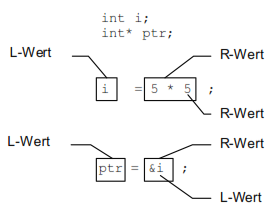
\includegraphics[width=1\textwidth]{pics/l-r-wert1.png}
		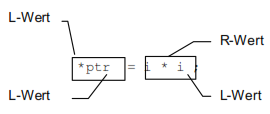
\includegraphics[width=1\textwidth]{pics/l-r-wert2.png}
	\end{minipage}
	
		\subsubsection{Zugriff auf L- und R-Werte}
			\begin{compactitem}
				\item Ein lvalue erfordert immer Schreibzugriff
				\item Auf einen rvalue wird nur lesend zugegriffen
				\item Es gibt auch nicht modifizierbare lvalues. Auf diese kann auch nur lesend zugegriffen werden.
			\end{compactitem}
	 
	\subsection{Operatoren im einzelnen}
		\begin{minipage}[t]{9 cm}
			\subsubsection{Bereichsoperator (Scope Operator) \lc{::}}
				Der Bereichs-Operator ist erst in \lc{C++} verf�gbar und liefert dem Compiler den Hinweis, in welchem Namespace er nach einem Symbol suchen soll. Der Namespace steht dabei links der beiden Doppelpunkte \lc{::} und der Symbolname steht rechts davon.
				
			\subsubsection{Un�re arithmetische Operatoren}
				\begin{compactitem}
					\item Positiver Vorzeichenoperator \lc{+A}
					\item Negativer Vorzeichenoperator \lc{-A}
					\item Postfix-Inkrementoperator \lc{A++}
					\item Pr�fix-Inkrementoperator \lc{++A}
					\item Postfix-Dekrementoperator \lc{A-\phantom{}-}
					\item Pr�fix-Dekrementoperator \lc{-\phantom{}-A}
				\end{compactitem}
				
			\subsubsection{Bin�re arithmetische Operatoren}
				\begin{compactitem}
					\item Additionsoperator \lc{A+B}
					\item Subtraktionsoperator \lc{A-B}
					\item Multiplikationsoperator \lc{A*B}
					\item Divisionsoperator \lc{A/B}
					\item Modulooperator \lc{A\%B}   
				\end{compactitem}
				
			\subsubsection{Zuweisungsoperatoren}
				\begin{compactitem}
					\item Zuweisungsoperator \lc{A=B}
					\item Kombinierte Zuweisungsoperatoren
					\begin{compactitem}
						\item Alle arithmetischen und logischen Operatoren haben zusammen mit dem
						Zuweisungsoperator eine verk�rzte Form, die das Schreiben verk�rzt (mehr nicht)
						\item Beispiel:\\
						\lc{a=a/b;}\\
						kann verk�rzt geschrieben werden als\\
						\lc{a/=b;}
					\end{compactitem}
				\end{compactitem}
				
			\subsubsection{Bit-Operatoren}
				\begin{compactitem}
					\item Bitweises AND \lc{A\&B}
					\item Bitweises OR \lc{A|B}
					\item Bitweises NOT (Inverter) \lc{\textasciitilde A}
					\item Bitweises XOR \lc{A\textasciicircum B} 
				\end{compactitem}
		\end{minipage}
		\hspace*{0.5cm}
		\begin{minipage}[t]{9 cm}
			\subsubsection{Relationale Operatoren\newline  (Vergleichsoperatoren)}
				\begin{compactitem}
					\item Gleichheitsoperator \lc{A==B}
					\item Ungleichheitsoperator \lc{A!=B}
					\item Gr�sseroperator \lc{A\textgreater B}
					\item Kleineroperator \lc{A\textless B}
					\item Gr�ssergleichoperator \lc{A\textgreater=B}
					\item Kleinergleichoperator \lc{A\textless=B} 
				\end{compactitem}	
				
			\subsubsection{Logische Operatoren}
				\begin{compactitem}
					\item Logisch UND (AND) \lc{A\&\&B}
					\item Logisch ODER (OR) \lc{A||B}
					\item Logisch NICHT (NOT) \lc{!A}\\
					0 = false, falsch\\
					1 = true, wahr (genauer: ungleich 0)
				\end{compactitem}	
				
			\subsubsection{Schiebe- (Shift-) Operatoren}
				\begin{compactitem}
					\item Rechts-Shift um n Bits \lc{A>\phantom{}>n}
					\item Links-Shift um n Bits \lc{A<\phantom{}<n}
				\end{compactitem}
				
				\subsubsection{Bedingungsoperator (Tern�rer Operator)}
					\lc{A?B:C} ist eine verk�rzte Schreibweise f�r
					\lstinputlisting[language=C,tabsize=2]{code/Ternaerer_Operator.c}
					
					Beispiel Maximum von zwei Zahlen a, b ermitteln:
					\lstinputlisting[language=C,tabsize=2]{code/Ternaerer_Operator2.c}
					entspricht:
					\lstinputlisting[language=C,tabsize=2]{code/Ternaerer_Operator3.c}
		\end{minipage}	

	\section{Anweisungen}

	\section{Funktionen}
	\subsection{Aufgaben einer Funktion}
		\begin{compactitem}
			\item Gleichartige, funktional zusammengeh�rende Programmteile unter einem eigenen Namen zusammenfassen. Der Programmteil kann mit diesem Namen aufgerufen werden.
			\item Einige Funktionen (im speziellen mathematische) sollen parametrisiert werden k�nnen, z.B. die Cosinusfunktion macht nur Sinn, wenn sie mit unterschiedlichen Argumenten aufgerufen werden kann.
			\item Divide et impera (divide and conquer, teile und herrsche): Ein grosses Problem ist einfacher zu l�sen, wenn es in mehrere einfachere Teilprobleme aufgeteilt wird. 
		\end{compactitem}	
		
	\subsection{Definition von Funktionen \verweisboth{9.3.1}{7.2}}
		\begin{minipage}[c]{10 cm}
			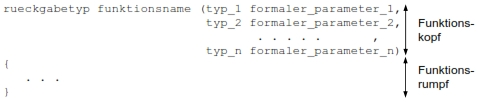
\includegraphics[width=1\textwidth]{pics/funktionen_aufbau.jpg}
		\end{minipage}
		%
		\begin{minipage}[c]{9 cm}
			\begin{compactitem}
				\item Funktionskopf: legt die Aufrufschnittstelle (Signatur) der Funktion fest. Er besteht aus R�ckgabetyp, Funktionsname und Parameterliste.
				\item Funktionsrumpf: Lokale Vereinbarungen und Anweisungen innerhalb eines Blocks
			\end{compactitem}	
		\end{minipage}	
			
	\subsection{Eingaben/Ausgaben einer Funktion \verweisboth{9.3}{7.3}}
		\begin{minipage}[t]{8.5 cm}
			\subsubsection{Eingabedaten}
				Es sind folgende M�glichkeiten vorhanden um Daten an Funktionen zu �bergeben:
				\begin{compactitem}
					\item Mithilfe von Werten, welche an die Parameterliste �bergeben werden
					\item Mithilfe von globalen Variablen
				\end{compactitem}
		\end{minipage}
		\hspace*{0.5cm}
		\begin{minipage}[t]{8.5 cm}
			\subsubsection{Ausgabedaten}
				Es sind folgende M�glichkeiten vorhanden um Daten zur�ckzugeben:
				\begin{compactitem}
					\item Mithilfe des R�ckgabewertes einer Funktion ($return$)
					\item Mithilfe von �nderungen an Variablen, deren Adresse �ber die Parameterliste an die Funktion �bergeben wurde
					\item Mithilfe von �nderungen an globalen Variablen
				\end{compactitem}	
		\end{minipage}	
		
		\subsubsection{Beispiele}
			\begin{minipage}[t]{8.5 cm}
				\textbf{Parameterlos und ohne R�ckgabewert:}
				\lstinputlisting[language=C,tabsize=2]{code/funktionen_parameter_1.c}
				
				\textbf{Parameter und ohne R�ckgabewert:}
				\lstinputlisting[language=C,tabsize=2]{code/funktionen_parameter_2.c}
			\end{minipage}
			\hspace*{0.5cm}
			\begin{minipage}[t]{8.5 cm}
				\textbf{Parameter und R�ckgabewert:}
				\lstinputlisting[language=C,tabsize=2]{code/funktionen_parameter_3.c}
			\end{minipage}

	\subsection{Deklaration von Funktionen \verweisboth{9.4}{7.2}}
		Es ist festgelegt, dass die Konsistenz zwischen Funktionskopf und Funktionsaufrufen vom Compiler �berpr�ft werden soll. Dazu muss beim Aufruf der Funktion die Schnittstelle der Funktion, d.h. der Funktionskopf, bereits bekannt sein. Steht aber die Definition einer Funktion im Programmcode erst nach ihrem Aufruf, so muss eine Vorw�rtsdeklaration der Funktion erfolgen, indem vor dem Aufruf die Schnittstelle der Funktion mit dem Funktionsprototypen deklariert wird. \\
		Desweitern ist zu beachten, dass Parameternamen im Funktionsprototyp und in der Funktionsdefinition nicht �bereinstimmen m�ssen. Es ist jedoch zu empfehlen.
		
		\begin{minipage}[t]{9.5 cm}
			\subsubsection{Beispiel}
				\lstinputlisting[language=C,tabsize=2]{code/funktionen_prototyp.c}	
		\end{minipage}
		\hspace*{0.5cm}
		\begin{minipage}[t]{7.5 cm}	
			\subsubsection{Was passiert wenn der Prototyp vergessen geht?}
				\begin{compactitem}
					\item Fehlt der Prototyp ganz, so wird die Funktion implizit (automatisch vom System) deklariert. Ihr R�ckgabetyp wird als $int$ angenommen, die Parameter werden nicht �berpr�ft.
					\item Wenn die Funktion sp�ter definiert wird und nicht $int$ als R�ckgabetyp hat, bringt der Compiler eine Fehlermeldung.
				\end{compactitem}
		\end{minipage}
		
		\subsubsection{Funktionsprototypen in der Praxis \verweisc{9.4}}
			\begin{compactitem}
				\item Funktionsprototypen, welche die Schnittstelle der Unit beschreiben, kommen in das entsprechenden Headerfile.
				\item Jedes C-File, welches diese Schnittstelle nutzt, inkludiert dieses Headerfile und somit die Funktionsprototypen.
				\item Funktionsprototypen von internen Funktionen der Unit werden zuoberst im C-File aufgelistet und kommen nicht ins Headerfile.
			\end{compactitem}
			
	\subsection{$inline$-Funktionen vs. $C$-Makros \verweiscpp{7.5}}
		\begin{minipage}[t]{7 cm}
			\subsubsection{$C$-Makros}
				\begin{compactitem}
					\item $C$-Makros werden definiert mit $\#define$.
					\item $C$-Makros bewirken eine reine Textersetzung ohne jegliche Typenpr�fung.
					\item Bei Nebeneffekten (welche zwar vermieden werden sollten) verhalten sich Makros nicht wie beabsichtigt.
					\item $C$-Makros l�sen zwar das Problem mit dem Overhead, sind aber sehr unsicher.				
				\end{compactitem}
				\lstinputlisting[language=C,tabsize=2]{code/c_makro.c}
			\end{minipage}
			\hspace*{0.5cm}
			\begin{minipage}[t]{10 cm}	
				\subsubsection{$inline$-Funktionen}
					\begin{compactitem}
						\item L�sen das Overhead-Problem.
						\item Der Code wird direkt eingef�gt, kein Funktionsaufruf findet statt.
						\item Eine Typenpr�fung wird durchgef�hrt.
						\item Einsetzen wenn der Codeumfang der Funktion sehr klein ist und die Funktion h�ufig aufgerufen wird (z.B. in Schleifen).
						\item Rekursive Funktionen und Funktionen, auf die mit einem Funktionspointer gezeigt wird, werden nicht $inlined$.
					\end{compactitem}
					\lstinputlisting[language=C++,tabsize=2]{code/inline.cpp}
			\end{minipage}	
		
	\subsection{Vorbelegte Parameter \verweiscpp{7.6}}
		\begin{compactitem}
		\end{compactitem}
	
	\section{H�here Datentypen und strukturierte Datentypen \verweiscpp{8}}  		
  	\subsection{Pointer \verweisboth{6}{8.2}}	
  \begin{minipage}[t]{7 cm}
  		\subsubsection{Arbeisspeicher - Memory Map \verweisc{6.1}}
  			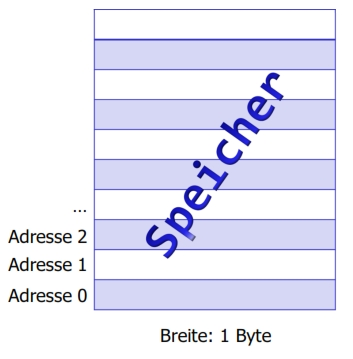
\includegraphics[width=0.8\textwidth]{pics/arbeitsspeicher.jpg}
  			
  			\begin{compactitem}
  				\item Der gesamte Speicher besteht aus einer Folge von einzelnen Bytes, welche durchnumeriert werden.
  				\item Diese eindeutige Nummer einer Speicherzelle wird als Adresse bezeichnet.
  				\item Bei einem byteweise adressierbaren Speicher (ist �blich) liegt an jeder Adresse genau 1 Byte.
  			\end{compactitem}
  	\end{minipage}
  	\hspace*{0.5cm}
  	\begin{minipage}[t]{10.5 cm}
  		\subsubsection{Pointer \verweisc{6.1}}
  			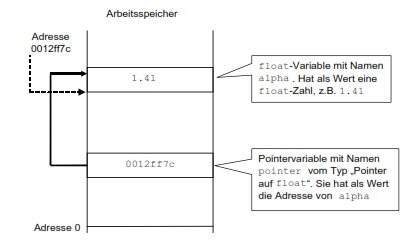
\includegraphics[width=0.95\textwidth]{pics/pointer.jpg}
  				
  			\begin{compactitem}
  				\item Ein Pointer ist eine Variable, welche die Adresse einer im Speicher befindlichen Variablen oder Funktion aufnehmen kann.
  				\item Man sagt, der Pointer zeige (to point) auf diese Speicherzelle.
  				\item Pointer in \lc{C} sind typisiert, sie zeigen auf eine Variable des definierten Typs.
  				\item Der Speicherbereich, auf den ein bestimmter Pointer zeigt, wird entsprechend des definierten Pointer-Typs interpretiert.
  				\item Der Speicherbedarf einer Pointervariablen ist unabh�ngig vom Pointer-Typ. Er ist so gross, dass die maximale Adresse Platz findet (z.B. 32 Bit).
  			\end{compactitem}
  	\end{minipage}	

	\begin{minipage}[t]{10 cm}
		\subsubsection{Definition einer Pointervariablen \verweisboth {6.1}{8.2.1}}		
			\vspace*{-0.3cm}\lstinputlisting[language=C,tabsize=2]{code/pointer_init.c}
	\end{minipage}
	\hspace*{0.5cm}
	\begin{minipage}[t]{8.5 cm}
		\subsubsection{Initialisierung mit Nullpointer \verweisc {6.1}}
			NULL ist vordefiniert (in \lc{stddef.h}) und setzt den Pointer auf einen definierten Nullwert. Besser ist es, statt \lc{NULL} direkt \lc{0} zu verwenden.
			\vspace*{-0.2cm}\lstinputlisting[language=C,tabsize=2]{code/pointer_null.c}
	\end{minipage}		
			
	\begin{minipage}[t]{9 cm}
		\subsubsection{Der Adressoperator (Referenzierung) \verweisboth {6.1}{8.2.2}}	
			Ist \lc{x} eine Variable vom Typ \lc{Typname}, so liefert der	Ausdruck \lc{\&x} einen Pointer auf die Variable \lc{x}, d.h. er liefert die Adresse der Variablen \lc{x}.	
			\lstinputlisting[language=C,tabsize=2]{code/pointer_adressoperator.c}
	\end{minipage}
	\hspace*{0.5cm}
	\begin{minipage}[t]{9 cm}
		\subsubsection{Der Inhaltsoperator * (Dereferenzierung) \verweisboth {6.1}{8.2.3}}
			Ist \lc{ptr} ein Pointer vom Typ \lc{Typname}, so liefert der	Ausdruck \lc{*ptr} den Inhalt der Speicherzelle, auf welche \lc{ptr} zeigt.
			\vspace*{-0.2cm}\lstinputlisting[language=C,tabsize=2]{code/pointer_inhaltsoperator.c}
	\end{minipage}	
	
	\subsubsection{Pointerarithmetik \verweisboth{10.1.1}{8.3.2}}
		\begin{minipage}[t]{9 cm}
			\textbf{Zuweisung:} 
			\begin{compactitem}
				\item Pointer unterschiedlicher Datentypen d�rfen einander nicht zugewiesen werden (Schutzmechanismus).
				\item Einem Pointer eines bestimmten Typs d�rfen Pointer dieses Typs oder \lc{void}-Pointer zugewiesen werden.
				\item Einem \lc{void}-Pointer d�rfen beliebige Pointer zugewiesen werden (n�tzlich aber gef�hrlich).
			\end{compactitem}
			\ \\
			\textbf{Vergleiche:} 
			\begin{compactitem}
				\item Bei Pointern desselben Typs funktionieren Vergleiche wie \lc{==}, \lc{!=}, \lc{<}, \lc{>}, \lc{>=}, etc.
				\item Hintergrund: ein Pointer ist eine Adresse, d.h. die Vergleiche passieren mit den Adressen. Daraus ist klar, was die Vergleiche bewirken.
			\end{compactitem}
		\end{minipage}	
		\hspace*{0.5cm}
		\begin{minipage}[t]{9 cm}
			\textbf{Addition und Subtraktion:} 
				\begin{compactitem}
					\item Zu einem Pointer darf eine ganze Zahl oder ein anderer Pointer desselben Typs addiert werden.
					\item Von einem Pointer kann eine ganze Zahl oder ein anderer Pointer desselben	Typs subtrahiert werden.
					\item Wenn eine ganze Zahl n addiert / subtrahiert wird, so bewegt sich der Pointer	auf das n�chste Element des Pointertyps. Die Zahl n wird also nicht als Byte interpretiert, der Pointer bewegt sich um \lc{n*sizeof(Typ)} Bytes.
				\end{compactitem}
				\ \\
				\textbf{Andere Operationen:} 
				\begin{compactitem}
					\item Andere Operationen sind nicht erlaubt!
				\end{compactitem}
		\end{minipage}	
	
	\subsubsection{Pointer auf void \verweiscpp{8.2.7}}
		\begin{minipage}[t]{5 cm}
			\lstinputlisting[language=C,tabsize=2]{code/voidptr.c}
		\end{minipage}
		\hspace*{0.5cm}
		\begin{minipage}[t]{13 cm}
			\begin{compactitem}
				\item Wenn bei der Definition des Pointers der Typ der Variablen, auf die der Pointer zeigen soll, noch nicht feststeht, wird ein Pointer auf den Typ \lc{void} vereinbart.
				\item Ein Pointer auf \lc{void} umgeht die Typenpr�fung des Compilers. Er kann einem typisierten Pointer zugewiesen werden aber er kann keine Zuweisung von einem typisierten Pointer erhalten (in \lc{C} erlaubt).
				\item Abgesehen von einem Pointer auf \lc{void}, darf ohne explizite Typenkonvertierung kein Pointer auf einen Datentyp an einem Pointer mit einem anderen Datentyp zugewiesen werden.
				\item Jeder Pointer kann durch Zuweisung in den Typ \lc{void*} und zur�ck umgewandelt werden, ohne dass Informationen verloren gehen.
			\end{compactitem}
 		\end{minipage}
\newpage       
		\subsubsection{Pointer auf Funktionen \verweisboth{10.8}{8.2.7}}
			\begin{compactitem}
				\item Jede Funktion befindet sich an einer definierten Adresse im Codespeicher.
				\item Diese Adresse kann ebenfalls ermittelt werden.
				\item Interessant w�re, dynamisch zur Laufzeit in Abh�ngigkeit des Programmablaufs eine unterschiedliche Funktion �ber einen Funktionspointer aufzurufen (z.B. um unterschiedliche Integrale zu berechnen).
			\end{compactitem}
			
			\begin{minipage}[t]{10 cm}
				\vspace*{-0.5cm}\lstinputlisting[language=C,tabsize=2]{code/pointer_funktion.c}
			\end{minipage}
			\hspace*{0.5cm}
			\begin{minipage}[t]{8 cm}
				\textbf{Vereinbarung eines Pointers}
					\lstinputlisting[language=C,tabsize=2]{code/pointer_funktion_vereinbarung.c}
					$ptr$ ist hier ein pointer auf eine Funktion mit R�ckgabewert vom Typ $int$ und einem �bergabeparameter vom Typ $char$. Die Klammern m�ssen unbedingt gesetzt werden. \\
				
				\textbf{Zuweisung einer Funktion}
					\lstinputlisting[language=C,tabsize=2]{code/pointer_funktion_zuweisung.c} \ \\
					
				\vspace*{-0.7cm}\textbf{Aufruf einer Funktion}
					\lstinputlisting[language=C,tabsize=2]{code/pointer_funktion_aufruf.c}
			\end{minipage}
             
       \begin{minipage}[t]{11 cm}
       		\subsubsection{Anlegen von dynamischen Objekten \verweiscpp{8.2.4}}
       			\vspace*{-0.4cm}\lstinputlisting[language=C,tabsize=2]{code/speicherverw.c}
		\end{minipage}
		\hspace*{0.5cm}
		\begin{minipage}[t]{7 cm}   		
       		\subsubsection{Zerst�ren von dynamischen Objekten \verweiscpp{8.2.5}}  
       			\lstinputlisting[language=C,tabsize=2]{code/speicherverw2.c}   		
       			C++ verf�gt �ber keine automatische Speicherverwaltung (garbage collection), explizit angeforderte Speicherstellen m�ssen daher mit delete freigegeben werden.
       \end{minipage}
       
		\subsubsection{const bei Pointern und Arrays \verweisboth{10.4}{8.2.6}}
			\begin{minipage}[t]{9 cm}
				\paragraph{const bei Pointer - konstanter Pointer}
					\lstinputlisting[language=C,tabsize=2]{code/const_pointer_2.c}
					Hier ist nun der Pointer \lc{text} konstant. Die Position von \lc{const} ist sehr	relevant! 						
			\end{minipage}
			\hspace*{0.5cm}
			\begin{minipage}[t]{9 cm}
				\paragraph{const bei Pointer - konstanter String}
					\lstinputlisting[language=C,tabsize=2]{code/const_pointer_1.c}
					Dies bedeutet nicht, dass der Pointer \lc{text} konstant ist, sondern dass \lc{text} auf einen konstanten String zeigt.
			\end{minipage} 

			\begin{minipage}[t]{9 cm}
				\paragraph{const bei Arrays}
					\lstinputlisting[language=C,tabsize=2]{code/const_array.c}
					\lc{arr[0]}, \lc{arr[1]} und \lc{arr[2]} sind alle konstant und k�nnen somit nach der Initialisierung nicht mehr abge�ndert werden.
			\end{minipage}
			\hspace*{0.5cm}
			\begin{minipage}[t]{9 cm}					
				\paragraph{const bei Pointer - konstanter Pointer auf konstanten String}
					\lstinputlisting[language=C,tabsize=2]{code/const_pointer_3.c}
					Bei dieser Variante ist sowohl der Pointer \lc{text} als auch der String, auf welchen \lc{text} zeigt, konstant. 
			\end{minipage} 
								
	\subsection{Vektoren \verweisboth{10.7.1}{8.3}}
			\begin{minipage}[c]{9 cm}
				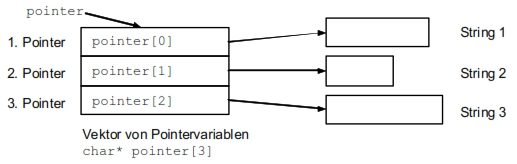
\includegraphics[width=1\textwidth]{pics/pointer_vektoren_1.jpg}
			\end{minipage}
			\hspace*{0.5cm}
			\begin{minipage}[c]{9 cm}
				Ein Pointer ist eine Variable, in der die Adresse eines anderen Speicherobjektes gespeichert ist. Entsprechend einem eindimensionalen Vektor von gew�hnlichen Variablen kann nat�rlich auch ein eindimensionaler Vektor von Pointervariablen gebildet werden.
			\end{minipage}
			
			\begin{minipage}[c]{9 cm}
				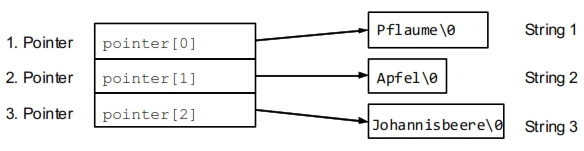
\includegraphics[width=1\textwidth]{pics/pointer_vektoren_2.jpg}
			\end{minipage}
			\hspace*{0.5cm}
			\begin{minipage}[c]{9 cm}
				Arbeitet man mit mehreren Zeichenketten, deren L�nge nicht von vorherein bekannt ist, so verwendet man ein Array von Pointern auf \lc{char}.
			\end{minipage}
			
			\begin{minipage}[c]{9 cm}
				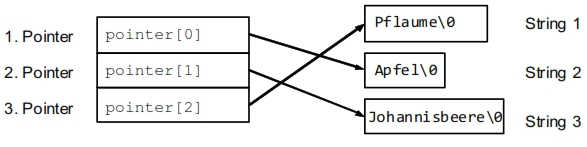
\includegraphics[width=1\textwidth]{pics/pointer_vektoren_3.jpg}
			\end{minipage}
			\hspace*{0.5cm}
			\begin{minipage}[c]{9 cm}
				Will man nun beispielsweise diese Strings sortieren, so muss dies nicht mit Hilfe von aufw�ndigen Kopieraktionen f�r die Strings durchgef�hrt werden. Es werden lediglich die Pointer so ver�ndert, dass die geforderte Sortierung erreicht wird.
			\end{minipage}
			
			\begin{minipage}[c]{9 cm}
				\lstinputlisting[language=C,tabsize=2]{code/pointer_vektoren.c}
			\end{minipage}
			\hspace*{0.5cm}
			\begin{minipage}[c]{9 cm}
				Formale Parameter f�r die �bergabe eines Arrays k�nnen in der Notation eines offenen Arrays ohne L�ngenangabe geschrieben werden. \lc{strPointer[]} ist demzufolge ein Vektor. Der Vektor besteht aus Pointern auf \lc{char}.
			\end{minipage}

		\begin{minipage}[t]{9 cm}
			\subsubsection{Initialisierung}
	  			\lstinputlisting[language=C,tabsize=2]{code/vec1.c}
		\end{minipage}	
		\hspace*{0.5cm}
		\begin{minipage}[t]{9 cm}  		
  			\subsubsection{Dynamische Allozierung}
    			\lstinputlisting[language=C,tabsize=2]{code/vec2.c}
    	\end{minipage}  	    			    	    			
    
	\subsection{Zeichenketten \verweisboth{10}{8.4}}
		\subsubsection{Initialisierung von Zeichenketten \verweisc{10.1.5 und Kapitel 10.1.6}}
			\lstinputlisting[language=C,tabsize=2]{code/string_init.c}
	
	\subsubsection{Kopieren eines Strings \verweisc{10.5}}
		\begin{minipage}[t]{9 cm}
			\paragraph{Variante mit Laufvariable}
				\vspace*{-0.5cm}\lstinputlisting[language=C,tabsize=2]{code/string_copy_manuell_1.c}
		\end{minipage}
		\hspace*{0.5cm}
		\begin{minipage}[t]{9 cm}
			\paragraph{Variante mit Pointer}
				\vspace*{-0.5cm}\lstinputlisting[language=C,tabsize=2]{code/string_copy_manuell_2.c}
		\end{minipage}
		
	\subsubsection{Standardfunktionen f�r Strings und Speicher \verweisc{10.6}}
		\begin{compactitem}
			\item Funktionen f�r die String- und Speicherverarbeitung sind prinzipiell dasselbe.
			\item Diese Funktionen werden in der Bibliothek \lc{string.h} zur Verf�gung gestellt.
			\item Funktionen die mit \lc{str} beginnen, dienen der Stringverarbeitung und erkennen das '\lc{$\backslash$0}'-Zeichen.
			\item Funktionen die mit \lc{mem} beginnen, dienen der Speicherverarbeitung und erkennen das '\lc{$\backslash$0}'-Zeichen nicht. 
		\end{compactitem}
		
		\begin{minipage}[t]{9 cm}
			\paragraph{String kopieren \verweisc {10.6.1.1}}
				\lstinputlisting[language=C,tabsize=2]{code/string_copy.c}
				\begin{compactitem}
					\item Dies Funktion kopiert einen String von \lc{src} nach \lc{dest} inklusive '\lc{$\backslash$0}'.
					\item Hat als R�ckgabewert den Pointer auf \lc{dest}.
					\item \lc{dest} muss auf einen Bereich zeigen, der gen�gend gross ist. Ist der zu kopierende Buffer gr�sser als der Zielbuffer, dann werden	nachfolgende Speicherbereiche �berschrieben (Buffer overflow).
				\end{compactitem}
				
			\paragraph{Strings zusammenf�gen \verweisc {10.6.1.2}}
				\lstinputlisting[language=C,tabsize=2]{code/string_concatenate.c}
				\begin{compactitem}
					\item Diese Funktion h�ngt einen String \lc{src} an \lc{dest} an, inklusive '\lc{$\backslash$0}'. Das urspr�ngliche '\lc{$\backslash$0} von \lc{dest} wird �berschrieben.
					\item Hat als R�ckgabewert den Pointer auf \lc{dest}.
					\item \lc{dest} muss auf einen Bereich zeigen, der gen�gend gross ist. Ist der zu kopierende Buffer gr�sser als der Zielbuffer, dann werden	nachfolgende Speicherbereiche �berschrieben (Buffer overflow).
				\end{compactitem}
		\end{minipage}
		\hspace*{0.5cm}
		\begin{minipage}[t]{9 cm}
			\paragraph{Strings vergleichen \verweisc {10.6.1.3}}
				\lstinputlisting[language=C,tabsize=2]{code/string_compare.c}
				\begin{compactitem}
					\item Dies Funktion vergleicht die beiden Strings, die auf \lc{s1} und \lc{s2} zeigen. Bei der Funktion \lc{strncmp} werden nur die ersten \lc{n} Zeichen verglichen.
					\item Dies Funktionen hat die folgenden R�ckgabewerte: \\
						\lc{<0} : \lc{*s1} ist lexikographisch kleiner als \lc{*s2} \\
						\lc{==0} : \lc{*s1} und \lc{*s2} sind gleich \\
						\lc{>0} : \lc{*s1} ist lexikographisch gr�sser als \lc{*s2}						
				\end{compactitem}
				
			\paragraph{Stringl�nge bestimmen \verweisc {10.6.1.5}}
				\lstinputlisting[language=C,tabsize=2]{code/string_length.c}
				\begin{compactitem}
					\item Diese Funktion bestimmt die L�nge von \lc{s}, d.h. die Anzahl der \lc{char}-Zeichen. Das '\lc{$\backslash$0}'-Zeichen wird dabei nicht mitgez�hlt.
					\item Hat als R�ckgabewert die L�nge von \lc{s}.
				\end{compactitem}
		\end{minipage} \\
		
		\begin{minipage}[t]{6 cm}
			\subsubsection{Funktionen zur Speicherbearbeitung \verweisc{10.6.2}}
				Die grunds�tzlichen Unterschiede zu den Stringfunktionen sind:
				\begin{compactitem}
					\item Formelle Parameter sind vom Typ \lc{void*} statt \lc{char*}.
					\item Die mem-Funktionen arbeiten byteweise.
					\item Im Gegensatz zu den \lc{str}-Funktionen wird das '\lc{$\backslash$0}'-Zeichen nicht speziell behandelt.
					\item Die Bufferl�nge muss als Parameter �bergeben werden.
				\end{compactitem}
		\end{minipage}
		\hspace*{0.5cm}
		\begin{minipage}[t]{12 cm}			
			\paragraph{Funktionen \verweisc{10.6.2.1 bis Kapitel 10.6.2.5}}
				\vspace*{-0.5cm}\lstinputlisting[language=C,tabsize=2]{code/mem_funktionen.c}
				Bei \lc{memcpy()} d�rfen sich die Buffer nicht �berlappen, \lc{memmove()} kann auch mit �berlappenden Buffern umgehen.\\
		\end{minipage} \\
		
\phantom{}

	\subsection{Referenzen \verweiscpp{8.1}}
		Referenzen sind alternative Namen oder Alias f�r ein Objekt. \\
		\begin{minipage}[t]{10.5 cm}
	  		\vspace*{-0.4cm}\lstinputlisting[language=C,tabsize=2]{code/ref1.c}
	  	\end{minipage}
	  	\begin{minipage}[t]{8 cm}	  		
			In 2 Situationen anwenden: 
  			\begin{compactitem}
  				\item Parameter�bergabe in Funktionen (call by Reference)
  				\item Referenz R�ckgabetyp anstatt Pointertyp (Objekte einer Klasse immer by reference �bergeben!)
  			\end{compactitem}
  			Niemals Pointer oder Referenz auf lokale Variable als \lc{return} Wert bei Funktionen. 
  		\end{minipage}	\\					
   
	\subsection{Pointer und Referenzen als R�ckgabewert und Parameter�bergabe \verweiscpp{8.6}}
  		Bei Variablen�bergabe (call by value) werden Kopien �bergeben, welche nicht ver�ndert werden k�nnen.\\
  		Bei Referenz�bergabe (call by reference) kann die Subroutine die Werte bleibend ver�ndern. \\
  		\begin{minipage}[t]{6 cm}
  			\subsubsection{call by reference}
   				\lstinputlisting[language=C,tabsize=2]{code/swap.c} 
   		\end{minipage}
    	\begin{minipage}[t]{6 cm}
      			\vspace*{0.6cm} \lstinputlisting[language=C,tabsize=2]{code/swap2.c} 
      	\end{minipage}
      	\begin{minipage}[t]{8 cm}
      		\subsubsection{call by value}
      	      	\lstinputlisting[language=C,tabsize=2]{code/swap3.c} 
      	\end{minipage}
    
	\subsection{Zugriff auf Class und Struct Elemente \verweiscpp{8.7}}
		\begin{minipage}[t]{7.5 cm}
			\lstinputlisting[language=C,tabsize=2]{code/classelem.c} 
		\end{minipage}
		\begin{minipage}[t]{11 cm}
			�hnlich wie bei Vektoren k�nnen nat�rlich auch die einzelnen Elemente von Klassen angesprochen werden. F�r den direkten Zugriff verwendet man die Operatoren \lc{.} und \lc{->}. \\
			Da es sich bei Klassen nicht um eine Aneinanderreihung von Elementen gleichen Types handelt, wird kein Index zur Adressierung der Elemente verwendet, sondern der Komponentenname. Der Unterschied zwischen den beiden Operatoren \lc{.} und \lc{->} besteht darin, dass \lc{.} auf eine Variable eines Klassentypes angewandt wird, w�hrend \lc{->} f�r Zeiger auf Klassentypen benutzt wird. \\
			Der Operator \lc{->} stellt nichts anderes als eine vereinfachte Schreibweise f�r eine Kombination von \lc{*} und \lc{.} dar: \\
			\lc{p->month = 12;} \\
			ist �quivalent zu: \\
			\lc{(*p).month = 12;}
		\end{minipage}


	\section{G"ultigkeitsbereiche, Namensr"aume und Sichtbarkeit}
\subsection{Namensr"aume und Sichtbarkeit}
\subsection{Deklarationen}
\subsection{Initialisierung}
\subsection{Type-cast}
\subsubsection{Standard-Typumwandlung}
Ausdr"ucke werden bei einer Zuweisung automatisch in erwarteten Typ umgewandelt.
\lstinputlisting[language=C,tabsize=2]{code/typecast.c} 
\subsubsection{explizite-Typumwadlung}
 M"ogliche Umwandlungen im C-Stil: (Problematisch)
 \lstinputlisting[language=C,tabsize=2]{code/typecast2.c}
		
	\section{Module und Datenkapseln \verweiscpp{10}}
	\begin{minipage}[t]{6.5 cm}
		\subsection{Motivation \verweiscpp{10.1}}
		\begin{compactitem}
			\item Arbeitsteilung: Grosse Programme werden von mehreren Personen entwickelt. Praktikabel ist, wenn nur eine Person an einer bestimmten Datei arbeitet.
			\item Effizienz: Eine �bersetzungseinheit (Datei) muss bei jeder �nderung neu �bersetzt werden (je gr�sser die Datei desto langsamer die �bersetzung)
			\item Strukturierung: Ein grosses Programm in mehrere vern�nftige Teile (Baugruppen, Units) aufteilen (Divide and conquer) 
			\linebreak
		\end{compactitem}
	\end{minipage}
	\hspace*{0.5cm}
	\begin{minipage}[t]{12 cm}
		\subsection{Nomenklatur Modul vs. Unit}
			\begin{compactitem}
				\item Ein Programmbaustein wird traditionell mit Modul bezeichnet
				\item Der Test eines Moduls heisst folglich Modultest
				\item Das Vorgehen, welches Module generiert, heisst Modularisierung 
				\item Heute �blicher wird Modul mit Unit, der Test mit Unittest bezeichnet, das Vorgehen heisst weiterhin Modularisierung 
			\end{compactitem}
		\subsection{Ziele der Modularisierung}
			\begin{compactitem}
				\item Klare, m�glichst schlanke Schnittstellen definieren
				\item Units so bilden, das Zusammengeh�rendes in einer Unit isoliert wird (Koh�sion soll hoch sein)
				\item Schnittstellen zwischen den Units sollen klein sein (Kopplung soll klein sein)
				\item Abh�ngigkeiten unter den Units sollen eine Hierarchie bilden, zirkul�re (gegenseitige) Abh�ngigkeiten m�ssen vermieden werden
			\end{compactitem}
	\end{minipage}

	\begin{minipage}[t]{10 cm}	
		\subsection{Vom Modul zur Datenkapsel \verweiscpp{10.2}}
			Eigenschaften einer Unit (eines Moduls):
			\begin{compactitem}	
				\item realisiert eine in sich abgeschlossene Aufgabe
				\item kommuniziert �ber ihre Schnittstelle mit der Umgebung
				\item kann ohne Kenntnisse ihres inneren Verhaltens in ein Gesamtsystem integriert werden (include Header)
				\item ihre Korrektheit kann ohne Kenntnis ihrer Einbettung in einem Gesamtsystem nachgewiesen werden (mittels Unittest)
				\item \textbf{Die Datenkapsel fordert nun zus�tzlich, dass auf die Daten nicht direkt zugegriffen werden darf, sondern nur �ber Zugriffsfunktionen.}
			\end{compactitem}
			Die Schnittstelle beschreibt, was das Modul zur Verf�gung stellt, verbirgt dabei wie das Verhalten konkret realisiert ist (Geheimnisprinzip, Information Hiding). Der User der Unit darf keine Annahme �ber den inneren Aufbau machen. Der Entwickler der Unit kann deren inneren Aufbau ver�ndern, solange die Schnittstelle dadurch nicht �ndert. 
	\end{minipage}
	\hspace*{0.5cm}
	\begin{minipage}[t]{8.5 cm}
		\subsection{Unitkonzept / Module und Datenkapseln in C++ \verweiscpp{10.3}}
		    \begin{compactitem}	
			  	\item Interface definiert die Schnittstelle, d.h. die Deklarationen wie Funktionsprototypen, etc. (Schaufenster)
			  	\item Implementation: in diesem Teil sind die Unterprogramme definiert, d.h. auscodiert (Werkstatt)
				 \item Das Interface wird in einer Headerdatei (*.h) beschrieben, die Implementation liegt in einer *.cpp- Datei
			\end{compactitem}
			\begin{center}
			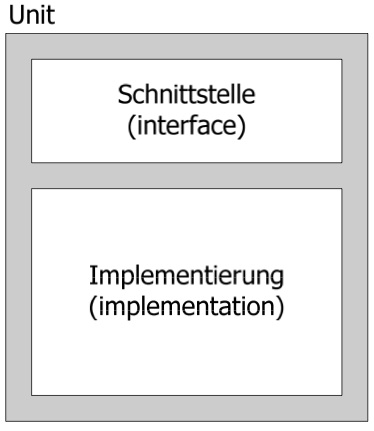
\includegraphics[width=0.28\textwidth]{pics/unit.jpg}
			\end{center}
	\end{minipage}

    \subsection{Die Schnittstellen-/Headerdatei \verweiscpp{10.3.1}}
		\begin{minipage}[t]{11 cm}
			 Jede .h-Datei enth�lt als erste Anweisungsfolge eine Include-Guard welche Mehrfacheinf�gen verhindert. Der Syntax lautet:
			 \lstinputlisting[language=C,tabsize=2]{code/includeguard.c}
			 Deklarationsreihenfolge in Headerdatei (*.h)  (Beispiel Kap 16.1)
			\begin{enumerate}
				\item Dateikommentar
				\item \#include der verwendeten System-Header (iostream, etc.) \newline
				      \#include <...>
				\item \#include der projektbezogenen Header (\#include "...")
				\item Konstantendefinitionen
				\item typedefs und Definition von Strukturen
				\item Allenfalls extern-Deklaration von globalen Variablen
				\item Funktionsprototypen, inkl. Kommentare der Schnittstelle, bzw. Klassendeklarationen
			\end{enumerate}
		\end{minipage}	
		\hspace*{0.5cm}
		\begin{minipage}[t]{7.5 cm}	
		  	\subsection{Beispiel Unit Rechteck}
		  	\lstinputlisting[language=c++,tabsize=2]{code/example_unit.cpp}
		\end{minipage}
\newpage
     	\begin{minipage}[t]{19 cm}
			\subsection{Die Implementierungsdatei \verweiscpp{10.3.2}}
				Deklarationsreihenfolge in Implementierungsdatei (*.cpp) (Beispiel Kap 16.1)
				\begin{enumerate}
			 		\item Dateikommentar
					\item \#include der verwendeten System-Header (iostream, etc.)
					      \#include <...>
					\item \#include der projektbezogenen Header (\#include "...") \newline
					      a) Hier k�me die Verwendung von $using$ $namespace$
					\item allenfalls globale Variablen und statische Variablen
					\item Pr�prozessor-Direktiven
					\item Funktionsprototypen von lokalen, internen Funktionen
					\item Definition von Funktionen und Klassen (Kommentare aus Headerdatei nicht wiederholen!!) 
					\linebreak
				\end{enumerate}
		\end{minipage}
		
		\subsection{Buildprozess / Makefile}
			\begin{minipage}[t]{11 cm}
			    Der Buildprozess erstellt aus den einzelnen Dateien einen ausf�hrbaren Code. Dazu werden zuerst alle *.cpp-Files compiliert.
			    Die daraus entstandenen Objektdatei m�ssen anschliessend gelinkt und somit zu einer auf�hrbaren Datei zusammengesetzt. Die Eingabe in der Konsole sieht wie folgt aus:
			    \lstinputlisting[language=C,tabsize=2]{code/compileUnit.c}
			    Es w�re m�hsam, wenn diese Befehle jedesmal neu eingetippt werden m�ssten. Deshalb wird in der Praxis oft ein Buildtool eingesetzt, z.B. make 
			 	\subsubsection{Make-File}
			 	\begin{compactitem}	
			 		\item In einem make-File k�nnen Abh�ngigkeiten definiert werden
			 		\item  Wenn eine Datei ge�ndert wurde, dann werden alle Operationen ausgef�hrt mit den Dateien, welche von dieser ge�nderten Datei abh�ngen
			 		\item Der Befehl (g++) wird z.B. nur dann ausgef�hrt, wenn sich an den Dateien, zu denen eine Abh�ngigkeit besteht, etwas ge�ndert hat
			 		\linebreak
				\end{compactitem}
				
			\end{minipage}
			\hspace*{0.5cm}
			\begin{minipage}[t]{7.5 cm}
				Abh�ngigkeitsliste gem�ss  UML-Notation:
				\linebreak
				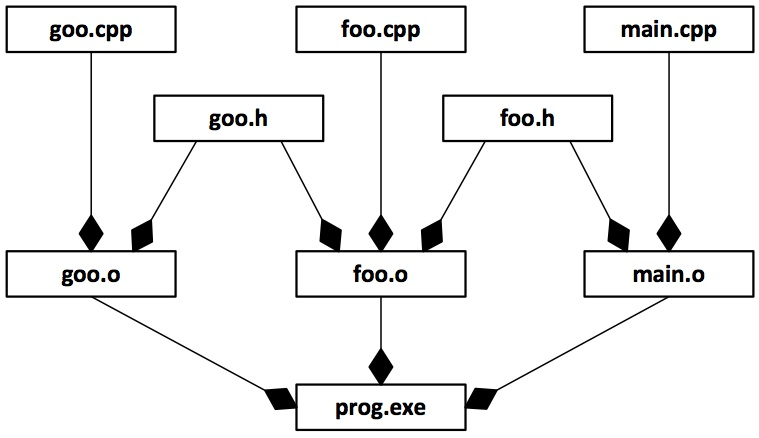
\includegraphics[width=1\textwidth]{pics/abhaengigkeitUML.jpg}
			    
			\end{minipage}
			\begin{minipage}[t]{19 cm}
			    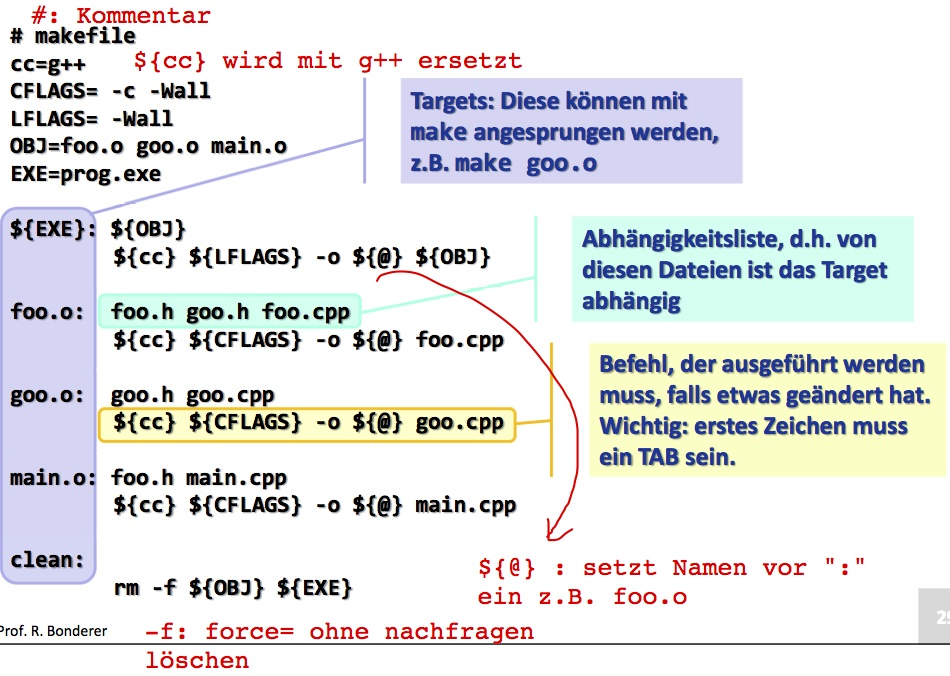
\includegraphics[width=0.6\textwidth]{pics/makefile.jpg}
			\end{minipage}
		
		

	
	\section{Klassenkonzept}
	\begin{minipage}[t]{7 cm}
		\subsection{Begriff der Klasse}
		\begin{compactitem}
			\item Eine Klasse ist eine Struktur (eine Struktur besteht nur aus Daten), die mit den 	Funktionen, welche auf diesen Daten arbeiten, erweitert wurde.
			\item Eine Klasse ist also eine Struktur, welche die Daten und die Funktionen auf diesen Daten in ein syntaktisches Konstrukt packt.
			\item Die Klasse ist die Umsetzung der Datenkapsel.
			\item Eine Klassendeklaration ist eine Typendefinition. Die Variablen einer Klasse
			werden als Objekte bezeichnet.
		\end{compactitem}
	\end{minipage}
	\hspace*{0.5cm}
	\begin{minipage}[t]{11 cm}
		\subsection{UML-Notation einer Klasse}
			\begin{tikzpicture}
				\begin{class}[text width=9.5cm]{ClassName}{0 ,0}
					\attribute {-attribute1: int = 0}
					\attribute {-attribute2: int = 0}
					\operation {+method1()}
					\operation {+method2()}
				\end{class}
			\end{tikzpicture}
			\begin{compactitem}
				\item Eine Klasse ist der Bauplan f�r Objekte.
				\item Eine Klasse besteht aus Daten (Attribute) und den Funktionen (Methoden) auf diesen Daten.
				\item Sichtbarkeit: 
				\begin{compactitem}
					\item $+$ : $public$
					\item $-$ : $private$
					\item $\#$ : $protected$
				\end{compactitem}
			\end{compactitem}
	\end{minipage}
	
	\begin{minipage}[t]{8 cm}	
		\subsection{�blicher Aufbau einer Klassensyntax \verweiscpp{11.1.1}}
			\lstinputlisting[language=C++,tabsize=2]{code/klassenschnittstelle.cpp} 
	\end{minipage}
	\hspace*{0.5cm}
	\begin{minipage}[t]{10 cm}		
			\subsubsection{Zugriffsschutz \verweiscpp{11.4}}
			\begin{compactitem}
				\item $public$ - Elemente k�nnen innerhalb und von ausserhalb der Klasse
				angesprochen werden.
					\begin{compactitem}
						\item fast alle Methoden sind $public$
						\item Attribute sollen nie $public$ sein
					\end{compactitem}
				\item $protected$ - Elemente k�nnen von innerhalb der Klasse und von abgeleiteten
				Klassen angesprochen werden.
					\begin{compactitem}
						\item nur sparsam einsetzen!
					\end{compactitem}
				\item $private$ - Elemente k�nnen nur innerhalb der Klasse angesprochen werden.
					\begin{compactitem}
						\item grunds�tzlich f�r alle Attribute und f�r einzelne (lokale) Methoden
					\end{compactitem}
			\end{compactitem}
	\end{minipage}
	
	\begin{minipage}[t]{9 cm}
		\subsubsection{Operationen einer Klasse}
			Operationen eine Klasse (= Funktionen, die im Klassenrumpf definiert sind) werden als
			Elementfunktionen oder Methoden bezeichnet.	�blicherweise beginnen Elementfunktionen mit einem Kleinbuchstaben und werden in camelCase (mixedCase) notiert.	
			\begin{lstlisting}[language=C++,tabsize=2]
				isEmpty();
			\end{lstlisting}	
	\end{minipage}
	\hspace*{0.5cm}
	\begin{minipage}[t]{9 cm}	
		\subsubsection{Information Hiding}
			\begin{compactitem}
				\item Klassen exportieren generell ausschliesslich Methoden. Alle Daten sind im Innern (private-Abschnitt) verborgen, der Zugriff erfolgt �ber die so genannten Elementfunktionen.
				\item Jede Klasse besteht damit aus zwei Dateien, der Schnittstellendatei ($.h$) und	der Implementierungsdatei ($.cpp$).
			\end{compactitem}
	\end{minipage}

\newpage
		\subsubsection{Beispiel an der Klasse Rechteck}
			\begin{minipage}[t]{9cm}
				\lstinputlisting[language=C++,tabsize=2]{code/class_rectangle_header.cpp}				
				\begin{tikzpicture}
					\begin{class}[text width=8cm]{Rectangle}{0 ,0}
						\attribute{-a : double}
						\attribute{-b : double}
						\operation{+setA(in newA : double)}
						\operation{+setB(in newB : double)}
						\operation{+getA() : double}
						\operation{+getB() : double}
						\operation{+getArea() : double}
					\end{class}
				\end{tikzpicture}
			\end{minipage}
			\hspace*{0.5cm}
			\begin{minipage}[t]{9 cm}
				\lstinputlisting[language=C++,tabsize=2]{code/class_rectangle.cpp} 
			\end{minipage}
			
	\begin{minipage}[t]{9cm}
		\subsection{Elementfunktionen \verweiscpp{11.2}}
			\begin{compactitem}
				\item sind Funktionen, die in der Schnittstelle der Klasse spezifiziert sind.
				\item Elementfunktionen haben vollen Zugriff auf alle Klassenelemente (auch auf
				solche, die mit private: gekennzeichnet sind.
				\item Auf Elementfunktionen kann nur unter Bezugnahme auf ein Objekt der Klasse, bzw. mit dem Scope-Operator (::) zugegriffen werden.
				\item Elementfunktionen sollen prinzipiell in der Implementierungsdatei (.cpp) implementiert werden. Dem Funktionsnamen muss dabei der Klassenname gefolgt von $::$ vorangestellt werden. (Beispiel: $int$ $Stack::pop()$)
			\end{compactitem}
	\end{minipage}
	\hspace*{0.5cm}
	\begin{minipage}[t]{9 cm}
			\subsubsection{Klassifizierung von Elementfunktionen}
				\begin{compactitem}
					\item Konstruktoren / Destruktoren
						\begin{compactitem}
							\item Konstruktor: erzeugen eines Objekts
							\item Destruktur: vernichten, freigeben eines Objekts
						\end{compactitem}
					\item Modifikatoren
						\begin{compactitem}
							\item �ndern den Zustand eines Objekts (Attribute �ndern)
						\end{compactitem}
					\item Selektoren
						\begin{compactitem}
							\item greifen nur lesend auf ein Objekt zu (immer const definieren!)
							\item Beispiel: $bool$ $Stack::isEmpty()$ $const;$
						\end{compactitem}
					\item Iteratoren
						\begin{compactitem}
							\item Erlauben, auf Elemente eines Objekts in einer definierten Reihenfolge	zuzugreifen
						\end{compactitem}
				\end{compactitem}
	\end{minipage}
		
	\begin{minipage}[t]{9cm}
			\subsubsection{$inline$-Funktionen \verweiscpp{11.2.1}}
				\begin{compactitem}
					\item Elementfunktionen, die innerhalb der Deklaration der Klassenschnittstelle (im	.h-File) implementiert sind, werden als (implizite) $inline$ - Funktionen
					behandelt.
					\item Elementfunktionen k�nnen in der Klassenimplementation explizit mit dem
					Schl�sselwort $inline$ gekennzeichnet werden.
					\item Implizite $inline$ - Funktionen verletzen zwar das Information Hiding Prinzip	und sollten deshalb grunds�tzlich vermieden werden.
					\item Jedoch: die impliziten $inline$ - Funktionen sind die Funktionen, die garantiert immer $inline$ verwendet werden (mit einigen wenigen
					Ausnahmen).
				\end{compactitem}	
	\end{minipage}
	\hspace*{0.5cm}
	\begin{minipage}[t]{9 cm}			
			\subsubsection{$const$-Elementfunktion \verweiscpp{11.2.2}}
				\begin{compactitem}
					\item Elementfunktionen, die den Zustand eines Objekts nicht �ndern (Selektoren)
					sollen explizit mit dem Schl�sselwort $const$ gekennzeichnet werden.
					\item Das Schl�sselwort $const$ muss sowohl im Prototypen als auch in der
					Implementierung geschrieben werden.
				\end{compactitem}
				\lstinputlisting[language=C++,tabsize=2]{code/elementfunktion_const.cpp} 
	\end{minipage}
\newpage	
	\begin{minipage}[t]{6cm}
			\paragraph{$mutable$ - Attribut}
				Ein Datenelement, das nie $const$ werden soll (auch nicht bei $const$-Elementfunktionen) kann	mit	$mutable$ gekennzeichnet werden.
				\lstinputlisting[language=C++,tabsize=2]{code/mutable.cpp}
	\end{minipage}
	\hspace*{0.5cm}
	\begin{minipage}[t]{12cm}			
		\subsection{$this$-Pointer \verweiscpp{11.3}}
			Der $this$-Pointer ist ein Pointer auf das eigene aktuelle Objekt, welches eine
			Methode aufgerufen hat.
			\lstinputlisting[language=C++,tabsize=2]{code/this_pointer.cpp}
	\end{minipage}
	
	\section{Templates}	
	
	\section{Vererbung (Inheritance)}
	Vererbung ist ein Konzept, das es erlaubt, neue Klassen auf Basis von alten Klassen zu definieren. Die neuen (Unter-, Sub-) Klassen besitzen, ohne Eingriffe in den
	Sourcecode der bereits bestehenden (Ober-, Basis-, Super-) Klassen, all deren Eigenschaften, sie $erben$ deren Verhalten und Daten. Den Vorgang der Vererbung nennt man $Ableiten$.\linebreak
	\begin{minipage}[t]{6.5 cm}
		\subsection{Einsatz der Vererbung \verweiscpp{13.1}}
		\begin{compactitem}
			\item Bestehende Klassen erweitern (zus�tzliche Attribute und Elementfunktionen)
			\item Bestehende Methoden einer Basisklasse �ndern (�berschreiben)
			\item Einsatz nur wenn eine \textbf{IST-EIN ("is a")} Beziehung besteht (z.B. Baum \textbf{ist eine} Pflanze, Blume \textbf{ist eine} Pflanze)
			\linebreak
		\end{compactitem}
		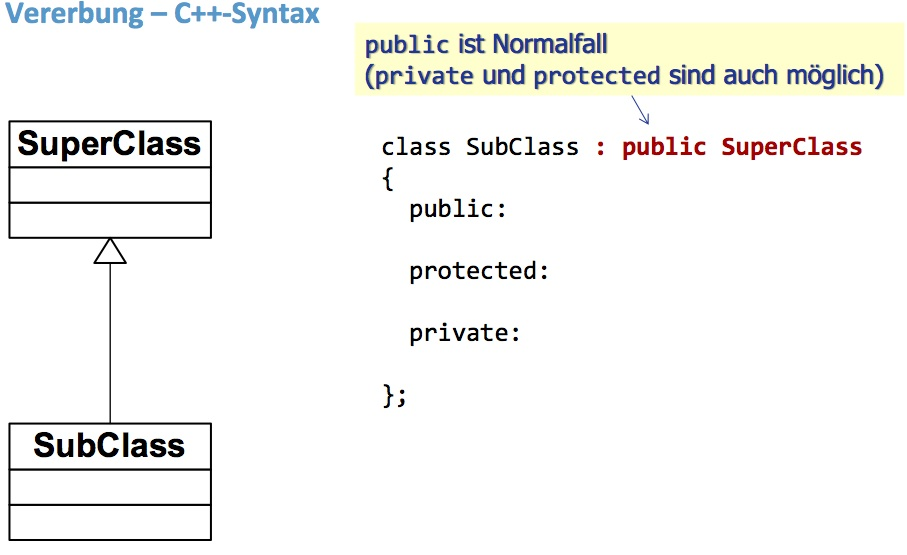
\includegraphics[width=1\textwidth]{pics/bsp_Vererbung.jpg}
		\subsection{Ableiten einer Klasse \verweiscpp{13.2}}
			Der Syntax der Ableitung einer Klasse ist oben aufgef�hrt. Als weiteres Beispiel ist im Anhang das Beispiel des ComicCharacters und SuperHero eingef�gt. SuperHero \textbf{ist ein} ComicCharacter.
			\begin{compactitem}
				\item friend-Beziehungen werden nicht vererbt
				\item Ein Objekt einer Oberklasse kann Objekte einer beliebigen Unterklasse aufnehmen
				\item Ein Objekt einer Unterklasse kann keine Objekte der Oberklasse aufnehmen
				\item Ein Objekt einer vererbten Klasse enth�lt alle Teile der Basisklasse und zus�tzlich noch die spezifischen eigenen Teile.
				\item Das Objekt ist somit mindestens so gross wie jenes der Basisklasse (es gibt keine Vererbung $by$ $reference$)
				\linebreak
			\end{compactitem}
				
	\end{minipage}	
	\hspace*{0.5cm}
	\begin{minipage}[t]{12 cm}
	\subsection{Zugriff auf Elemente der Basisklasse \verweiscpp{13.6}}
		\textbf{Bei Vererbung mit public (Normalfall):}
			\begin{compactitem}
				\item Zugriff m�glich auf alle public- und protected- Elemente der Basisklasse, die Zugriffsrechte 
				(public, protected) der Basisklasse werden in der abgeleiteten Klasse beibehalten
				\item kein Zugriff auf private-Elemente der Basisklasse
				\linebreak
			\end{compactitem}
		\textbf{Bei Vererbung mit protected:}
			\begin{compactitem}
				\item Zugriff m�glich auf alle public- und protected- Elemente der Basisklasse, die Zugriffsrechte 
				von public und protected der Basisklasse werden in der abgeleiteten Klasse zu protected
				\item kein Zugriff auf private-Elemente der Basisklasse
				\linebreak
			\end{compactitem}
		\textbf{Bei Vererbung mit private:}
			\begin{compactitem}
				\item Zugriff m�glich auf alle public- und protected- Elemente der Basisklasse, die Zugriffsrechte 
				von public und protected der Basisklasse werden in der abgeleiteten Klasse zu private
				\item kein Zugriff auf private-Elemente der Basisklasse
				\linebreak
			\end{compactitem}
	\subsection{Slicing Problem \verweiscpp{13.3}}
		Links: Beim Kopieren werden nur die ComicCharacter-Teile ber�cksichtigt. Durch das Kopieren wird alles �berfl�ssige weggeschnitten, �brig bleibt ein reines ComicCharacter Objekt im Fall von s f�hrt dies dazu, dass die erweiterten SuperHero Daten und Funktionen verloren gehen.\newline
		Rechts: Hier wird dank des Referenzparameters der gesamte Superheld ausgegeben.\newline
		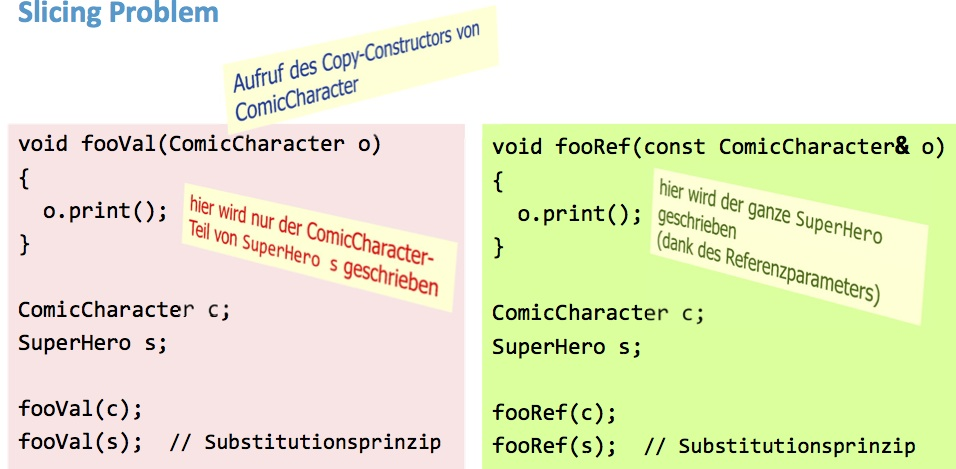
\includegraphics[width=1\textwidth]{pics/SlicingProblem.jpg}
	\end{minipage}	
	
	
	\section{Polymorphismus / Mehrfachvererbung / RTTI}
   	\begin{flushleft}
   	Dieses Kapitel beschreibt die dynamischen objektorientierten Sprachmerkmale von C++. Erst durch diese wird C++ zu einer echten objektorientierten Programmiersprache.
   	\end{flushleft}
	\begin{minipage}[t]{8 cm}
		\subsection{Polymorphismus \verweiscpp{14.1}}
			\subsubsection{dynamische vs. statische Bindung}
			Werden von einer Kasse A die Klassen B und C abgeleitet, so k�nnen Objekte vom Typ $Zeiger auf A$ auch auf B- oder C-Objekte verweisen. Implementieren alle drei Klassen eine Operation foo jeweils verschieden so bewirkt die Anweisung
			\lstinputlisting[language=C++,tabsize=2]{code/foo_poly.cpp}
			in normalen Programmiersprachen den Aufruf von $A::foo()$. Dabei wird bereits zur �bersetzungszeit (so fr�h wie m�glich; Early Binding) vom Compiler die Funktion $foo$ der Klasse A eingebunden. Diese Art des Bindens wird statische Bindung (static binding) genannt, da sie unver�nderbar ist. Die Variable $anAPointer$ kann in C++ auch f�r Objekte der Klasse B oder C stehen. \linebreak
			In echten objektorientierten Programmiersprache wird der obige Aufruf nicht zur �bersetzungszeit, sondern erst zur Laufzeit gebunden (dynamische Bindung, dynamic Binding). Beim Aufruf von \lstinputlisting[language=C++,tabsize=2]{code/foo_poly.cpp} wird der Typ des Objekts untersucht. In Abh�ngigkeit davon wird die Methode $A::foo$, $B::foo$ oder $C::foo$ aufgerufen. Dieses dynamische Verhalten wird als Polymorphismus bezeichnet. Damit dynamisch (zur Laufzeit) die verschiedenen Funktionen foo aufgerufen werden k�nnen, m�ssen diese Funktionen $virtual$ sein. \linebreak
	\end{minipage}\hspace*{0.5cm}
	\begin{minipage}[t]{10.5 cm}
		\subsection{Virtuelle Elementfunktionen \verweiscpp{14.2}}
			Virtuelle Elementfunktionen sind spezielle Funktionen, die nicht zur �bersetzungs- sondern zur Laufzeit gebunden werden. Es wird erst beim Auruf der Funktion entschieden, welche tats�chlich ausgef�hrt wird $A::foo$, $B::foo$ oder $C::foo$
				\begin{compactitem}
					\item Funktionen, die dynamisch gebunden werden, muss bei der Deklaration das Schl�sselwort virtual vorangestellt werden (zwingend!).
					In der abgeleiteten Klasse soll (muss aber nicht) die Funktion auch mit virtual gekennzeichnet werden. Dies sieht wie folgt aus:
						\lstinputlisting[language=C++,tabsize=2]{code/virtual.cpp}
					\item Faustregel: Eine Funktion sollte als virtual deklariert werden, wenn sie in der abgeleiteten Klasse neu definiert (�berschrieben) wird, sonst nicht!
					\item Achtung: nicht mit Funktions�berladung (gleicher Name aber unterschiedliche Signatur) verwechseln
					\item Die neue (�berschriebene) Methode muss dieselbe Signatur wie die Methode der Basisklasse haben. Sonst wird neue Methode eingef�hrt.
					\linebreak
				\end{compactitem}
	\end{minipage}
	\begin{minipage}[t]{5.5 cm}
	Im Beispiel rechts wird die Verwendung klar:
			\begin{compactitem}
				\item Der statische Datentyp bezeichnet den Datentyp bei der Deklaration. Im Beispiel: a ist ein Array von Pointer auf Article
				\item Der dynamische Datentyp bezeichnet den effektiven Datentyp zur Laufzeit Im Beispiel: a[0] ist ein Pointer auf Book, a[1] ein Pointer auf CD, etc.
			\end{compactitem}
	\end{minipage}
	\hspace*{0.5cm}
	\begin{minipage}[t]{13 cm}
		-\linebreak
		\includegraphics[width=1\textwidth]{pics/bsp_Webshop.jpg}
	\end{minipage}
\newpage
	\subsubsection{Aufruf von virtuelle Elementfunktionen \verweiscpp{14.2.2}}
	\begin{minipage}[t]{9 cm}
		Eine dynamische Methodenaufl�sung erfolgt �ber Zeiger oder Pointer:
		\lstinputlisting[language=C++,tabsize=2]{code/dynamic_call.cpp}
	\end{minipage}\hspace*{0.5cm}
	\begin{minipage}[t]{9 cm}
		Ein Aufruf mit einem Objekt und der Punktnotation wird statisch aufgel�st:
		\lstinputlisting[language=C++,tabsize=2]{code/static_call.cpp}
		Dies kommt daher, dass ein echtes Objekt sein Typ nicht ver�ndern kann (nicht polymorph) und der Compiler somit schon zur �bersetzungszeit entscheidet welche Funktion aufgerufen wird.
	\end{minipage}
	\begin{flushleft}
		Eine statische Aufl�sung wird auch erzwungen, wenn der G�ltigkeitsbereich explizit angegeben wird:
	\end{flushleft}
		\lstinputlisting[language=C++,tabsize=2]{code/static_call2.cpp}
	\begin{flushleft}
		Wichtig ist auch: innerhalb von Konstruktoren und Destruktoren \textbf{alle} Methodenaufrufe \textbf{statisch} aufgel�st werden. 
	\end{flushleft} 
	\begin{minipage}[t]{6 cm}
		\subsubsection{Polymorphe (virtuelle) Klassen}
			\begin{compactitem}
	 		\item Eine Klasse, welche mindestens eine virtuelle Funktion deklariert, heisst virtuell 	(polymorph)
			\item Virtuelle Klassen bewirken einen Mehraufwand f�r den Compiler und sind darum langsamer in der Ausf�hrung
			\item Konstruktoren sind nie virtuell
			\item Destruktoren virtueller Klassen m�ssen immer als virtuell deklariert werden,
			sonst wird nur der Destruktor der Basisklasse aufgerufen
			\textbf{ \item Nicht virtuelle Methoden d�rfen nicht �berschrieben werden} (k�nnten technisch gesehen, f�hrt aber zu un�berschaubaren Fehlern)
			\end{compactitem}
	
	\end{minipage}\hspace*{0.5cm}
	\begin{minipage}[t]{12.5 cm}
		\subsubsection{Repr�sentation polymorpher Objekte im Speicher \verweiscpp{14.2.6}}
			\begin{compactitem}
				\item In der Virtual Function Table (vtbl) vermerkt das System der Reihe nach die Adressen der f�r eine Klasse g�ltigen virtuellen Elementfunktionen
				\item Das System legt f�r jede polymorphe Klasse eine vtbl an
				\item Jedes Objekt einer polymorphen Klasse enth�lt einen Virtual Pointer vptr,
						welcher auf die vtbl der entsprechenden Klasse zeigt
			\end{compactitem}
		\hspace*{0.5cm}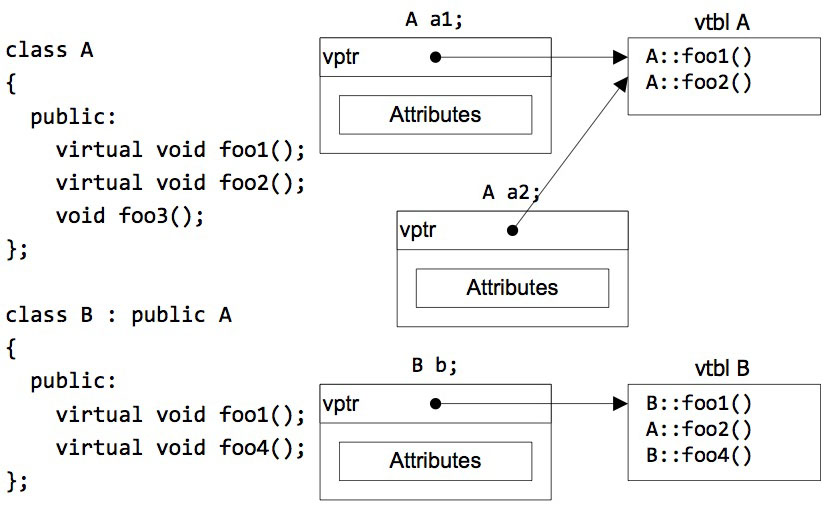
\includegraphics[width=0.85\textwidth]{pics/bsp_vtbl.jpg}
	\end{minipage}
	\subsection{Abstrakte Klassen \verweiscpp{14.3}}
		Eine abstrakte Klasse ist ein Klasse, die mehr oder weniger vollst�ndig ist und dazu dient, Gemeinsamkeiten der abgeleiteten Klassen festzuhalten (z.B. ComicCharacter). ComicCharacter legt fest, dass alle Comicfiguren die Methoden $print()$, $dance()$ und $sing()$ verstehen.
		\begin{compactitem}
			\item Ein Kreis ist z.B. ein Spezialfall einer Ellipse. Es ist aber nicht sinnvoll, ihn so zu programmieren, da er sonst Eigenschaften erbt, die nicht verwendet werden
			\item Es w�re m�glich, Kreis und Ellipse als zwei unabh�ngige Klassen zu programmieren. Dann m�ssten aber alle Eigenschaften, die diese gemeinsam haben, doppelt programmiert werden
			\item Dies versucht die objektorientierte Programmierung zu vermeiden
			\item Es ist besser, die Eigenschaften, die Kreise und Ellipsen gemein haben, in einer Basisklasse zu programmieren
			\item Die Kreis- und Ellipsenklasse erben dann parallel von der gemeinsamen Basisklasse
			\item Die Basisklasse ist aber unvollst�ndig, es handelt sich um eine abstrakte Klasse
			\item Es k�nnen \textbf{keine} Objekte von abstrakten Klassen gebildet werden
			\item In C++ k�nnen rein virtuelle Funktionen (pure virtual functions) deklariert werden, die in der Basisklasse nicht von einer Definition begleitet werden
			\lstinputlisting[language=C++,tabsize=2]{code/pure_virtual_function.cpp}
			\textbf{\item Klassen, die mindestens eine rein virtuelle Funktion deklarieren, sind abstrakte Klassen}
			\item Ist eine Klasse erst einmal als abstrakt definiert, kann diese nur durch Vererbung vervollst�ndigt und dadurch nutzbar gemacht werden \linebreak
		\end{compactitem}
		\begin{minipage}[t]{9 cm}
			So ist die folgende Klasse eine abstrakte Klasse (da mind. 1 Funktion rein virtuell ist)
			\lstinputlisting[language=C++,tabsize=2]{code/virtual_function.cpp}
		\end{minipage}\hspace*{0.5cm}
		\begin{minipage}[t]{9.5 cm}
			Der folgende Aufruf f�hrt daher beim �bersetzen zu einem Fehler. (Es k�nnen keine Objekte aus abstrakten Klassen erstellt werden)
			\lstinputlisting[language=C++,tabsize=2]{code/virtual_function2.cpp}
		\end{minipage}
	\subsection{Mehrfachvererbung \verweiscpp{14.3}}
		\begin{minipage}[t]{7.5 cm}
		Bei der Mehrfachvererbung wird eine Klasse von mehreren Basisklassen abgeleitet. So kann z.B. eine Klasse DuckHero definiert werden, die sowohl von SuperHero als auch von SingingComicCharacter erbt. \linebreak[2]
		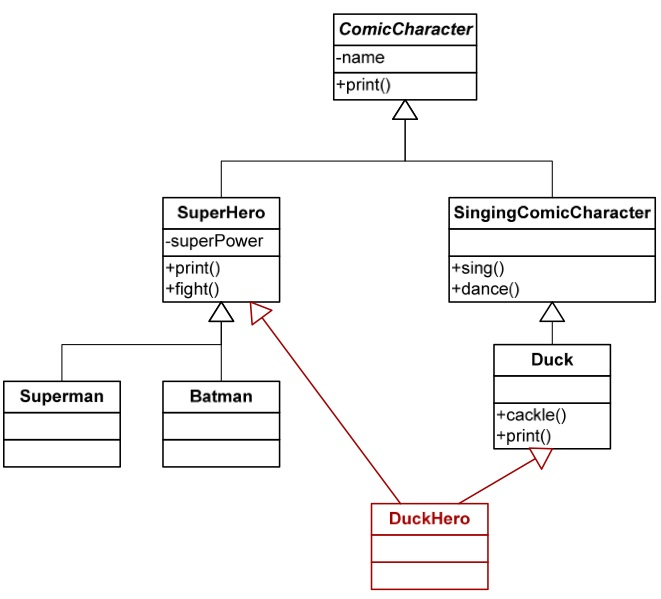
\includegraphics[width=1\textwidth]{pics/uml_mehrfachvererbung.jpg}
		Guter Einsatz der Mehrfachvererbung ist, wenn alle ausser h�chstens einer Basisklasse ausschliesslich aus rein virtuellen Funktionen bestehen (Interfaces). Die neue Klasse implementiert dann die aufgelisteten Interfaces.\linebreak
		Das obige Beispiel ist im Anhang unter 15.4 angeh�ngt.
		\end{minipage}\hspace*{0.5cm}
		\begin{minipage}[t]{11 cm}
		Der Syntax bei der Mehrfachvererbung lautet wie folgt (Basisklassen durch Komma getrennt): \linebreak
			\lstinputlisting[language=C++,tabsize=2]{code/mehrfachvererbung.cpp}
		Durch die Mehrfachverbung treten oft Probleme auf. Problem 1 ist jenes der Mehrdeutigkeit von Methoden. Im Fall von $print()$ ergeben sich mehrere M�glichkeiten. Um die Mehrdeutigkeit zu umgehen, muss der G�ltigkeitsbereich angegeben werden:
			\lstinputlisting[language=C++,tabsize=2]{code/mehrdeutigkeit.cpp}
		Oder noch besser:
			\lstinputlisting[language=C++,tabsize=2]{code/mehrdeutigkeit2.cpp}
		Das Problem 2 ist das von mehrfachen Basisklassen (linker und rechter Baum). DuckHero ist von Duck und SuperHero abgeleitet und beinhaltet somit zwei ComicCharacter-Teile. Diese Mehrdeutigkeit kann durch virtuelle Basisklassen verhindert werden (siehe Kap. 14.5 im Buch)
		\end{minipage}
\newpage
	\subsection{RTTI (Laufzeit-Typinformation) \verweiscpp{14.3}}
	RTTI (Run-Time Type Information) ist die M�glichkeit den Typ eines Objekts einer polymorphen Klasse festzustellen. Er steht ausschliesslich f�r polymorphe Klassen zur Verf�gung und sollte sehr zur�ckhaltend eingesetzt werden.\linebreak
	Der RTTI-Mechanismus besteht im Wesentlichen aus zwei Operatoren und einer Struktur:
		\begin{compactitem}
			\item Operator dynamic\_cast
			\item Operator typeid
			\item Klasse type\_info
		\end{compactitem}
	\subsubsection{Operator dynamic\_cast}
	Syntax: 	\lstinputlisting[language=C++,tabsize=2]{code/dynamic_cast.cpp}
		\begin{compactitem}
			\item Versucht, den Zeiger p in einen Zeiger auf ein Objekt des Typs SuperHero
			umzuwandeln
			\item Der dynamische Datentyp von p ist massgebend
			\item Umwandlung wird dann durchgef�hrt, wenn p tats�chlich auf ein Objekt vom Typ SuperHero, bzw. auf eine davon abgeleitete Klasse zeigt.
			\item Andernfalls ist das Resultat der Umwandlung der Nullpointer!
		\end{compactitem}
	\subsubsection{Operator typeid}
		\begin{compactitem}
			\item Ermitteln des dynamischen Datentyps eines polymorphen Objekts
			\item Ergibt eine Referenz auf ein Objekt des Typs $type\_info$. Diese Klasse beinhaltet u.a. eine Methode name(), welche den Namen der Klasse zur�ckgibt.
		Beispiel: \lstinputlisting[language=C++,tabsize=2]{code/typeid.cpp}
		\end{compactitem}
	\subsubsection{Struktur type\_info}
		Die Struktur muss eingebunden werden
		\lstinputlisting[language=C++,tabsize=2]{code/type_info.cpp}
		Sie bietet mind. folgende Funktionalit�t:
		\begin{compactitem}
			\item die Operatoren $==$ und $!=$
			\item die Methode $before$
			\item die Methode $name$ (siehe Beispiel oben)
		\end{compactitem}
	
	
	
	
		
	
	\section{Exception Handling \verweiscpp{15}}
	\begin{minipage}[t]{7 cm}
		\subsection{Exception vs. Error}
			\begin{compactitem}
				\item Error: Abweichung zur Spezifikation ("falsch implementiert").	Errors sollten bei der Verifikation (Testen) entdeckt und eliminiert werden.
				\item Exception: abnormale (aber vorhersehbare und m�gliche) Bedingung bei der
				Programmausf�hrung.
			\end{compactitem}			
	\end{minipage}
	\hspace*{0.5cm}
	\begin{minipage}[t]{11 cm}
			\subsubsection{M�gliche Reaktionen auf Ausnahmen \verweiscpp{15.1}}
				\begin{compactitem}
				 	\item Ignorieren: Motto: Augen zu und durch, eine sehr risikoreiche Variante.
				 	\item Programmabbruch: 	Merkt immerhin, dass etwas nicht in Ordnung ist, die Reaktion ist aber unbefriedigend. Ist Exception Detection aber nicht eigentlich Exception Handling.
				 	\item Exceptioncodes (nicht Fehlercodes): Funktionen geben als R�ckgabewert, als Parameter oder global einen	Ausnahmecode an.
				\end{compactitem}
	\end{minipage}
		
	\begin{minipage}[t]{7 cm}
		\subsection{Exceptionhandling in $C++$ \verweiscpp{15.2}}
			\begin{compactitem}
				\item Exceptions werden in Form eines Objekts am Ort ihres Auftretens ausgeworfen (explizit oder auch "automatisch").
				\item Exception Handler versuchen, diese Exception-Objekte aufzufangen.
			\end{compactitem}
			
			\subsubsection{Ausl�sen (Werfen) von Ausnahmen}
				\begin{compactitem}
					\item Ausnahmen k�nnen mit dem Schl�sselwort $throw$ explizit ausgeworfen werden.
					\item Nach einem $throw$-Befehl wird das Programm abgebrochen und beim ersten passenden umgebenden Handler fortgesetzt.
					\item Dabei werden alle lokalen Objekte wieder automatisch zerst�rt (Stack unwinding).
					\item Geworfen werden kann ein beliebiges Objekt (�blich: ein spezifisches Ausnahmeobjekt).
					\item (Ausschliesslich) innerhalb eines Exception Handlers ist auch die Form
					$throw;$ erlaubt. Dadurch wird die Exception an den	n�chsten Handler weitergereicht (Exception propagation).
				\end{compactitem}	
	\end{minipage}
	\hspace*{1cm}
	\begin{minipage}[t]{11 cm}
		\lstinputlisting[language=C++,tabsize=2]{code/exception_handling.cpp}
	\end{minipage}
	
	\begin{minipage}[t]{9 cm}
		\subsubsection{Exception-Hierarchie in $C++$}
			\vspace*{-0.4cm}\verweiscpp{15.4} \\ 		 	
			Ausnahmeobjekte k�nnen beliebigen Typs sein (z.B. auch int). Meist werden jedoch spezifische hierarchisch organisierte Ausnahmeklassen verwendet.
			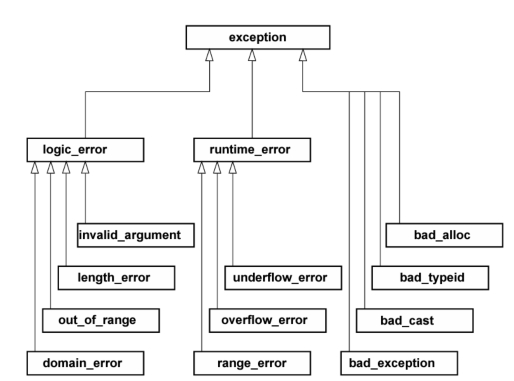
\includegraphics[width=0.8\textwidth]{pics/exception.jpg}
	\end{minipage}
	\hspace*{0.5cm}
	\begin{minipage}[t]{9 cm}
		\subsubsection{Laufzeit- vs. Logische Fehler}
			\begin{compactitem}
				\item Logische "Fehler" (logic\_error)
				\begin{compactitem}
					\item Ausnahmen im Programmablauf, die bereits zur Entwicklungszeit ihre Ursache	haben.
					\item Theoretisch k�nnten diese Ausnahmen verhindert werden.
				\end{compactitem}
				\item Laufzeit "Fehler" (runtime\_error)
				\begin{compactitem}
					\item Nicht vorhersehbare (?) Ausnahmen wie z.B. arithmetische �berl�ufe.
					\item Diese Ausnahmen treten erst zur Laufzeit auf, z.B. durch eine nicht erlaubte Benutzereingabe.
				\end{compactitem}
			\end{compactitem}
	\end{minipage}
	
	\begin{minipage}[t]{9 cm}
		\subsubsection{Excpetions und ihre Header}
			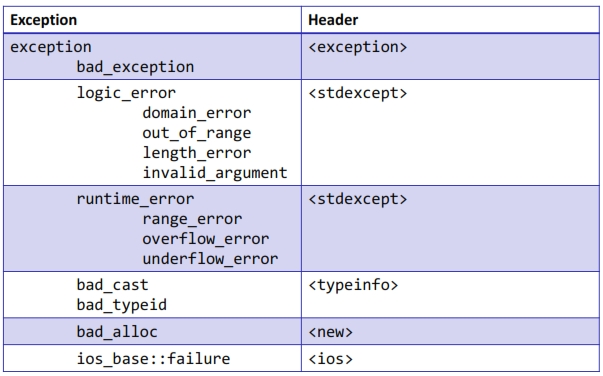
\includegraphics[width=1\textwidth]{pics/exception_header.jpg}
	\end{minipage}
	\hspace*{0.5cm}
	\begin{minipage}[t]{9 cm}
		\subsubsection{Exception Handler \verweiscpp{15.5}}
			\begin{compactitem}
				\item Ein oder mehrere Exception Handler k�nnen hintereinander definiert werden.
				\item Die einzelnen $catch$-Handler m�ssen sich in den Parametern unterscheiden.
				\item Wenn eine Exception geflogen kommt, wird der erste passende Handler
				genommen. Ein passender Handler macht ein $catch$ auf genau diese Exception oder auf eine Basisklasse derselben.
				\item Deshalb (sehr wichtig): Der allgemeinste Handler (am meisten oben in der Hierarchie) muss als letzter definiert werden.
			\end{compactitem}
	\end{minipage} \\
	
		\begin{minipage}[t]{9 cm}
			\paragraph{Aufruf}
				\begin{compactitem}
					\item Wenn kein Handler passt, dann wird im Aufrufstack nach oben gesucht, ob ein	passender Handler vorhanden ist.
					\item Wenn auch dort keiner gefunden wird, dann wird die Funktion $terminate()$ aufgerufen.
					\item $terminate($) beendet das Programm, kann aber auch selbst definiert werden.
					\item Catch all: Der folgende Handler f�ngt ausnahmslos alle Exceptions ab (und muss wenn gew�nscht deshalb immer als letzter aufgef�hrt werden):\\
					$catch(...)$\\
					$\{$\\
					$\}$\\					
				\end{compactitem}
		\end{minipage}
		\hspace*{0.5cm}
		\begin{minipage}[t]{9 cm}				
			\paragraph{Exception Specification}
				$void$ $foo()$ $throw(/*$ $Liste$ $der$ $Exceptions$ $*/);$
				\begin{compactitem}
					\item Liste beschreibt, welche Exceptions von einem Aufrufer von $foo()$ erwartet werden m�ssen.
					\item Aber: garantiert auch, dass das Programm abst�rzt, wenn eine andere als die	spezifizierten Exceptions ausgeworfen wird, d.h. $foo()$ muss daf�r sorgen, dass wirklich nur die aufgelisteten Exceptions ausgeworfen werden.
					\item Genauer: falls eine nicht spezifizierte Exception ausgeworfen wird, dann wird die Funktion $unexpected()$ aufgerufen, welche �blicherweise das Programm abbricht.
					\item $unexpected()$ kann selbst definiert werden.
				\end{compactitem}
		\end{minipage}
		
	\subsection{Handling Strategie von System Exceptions}
		\begin{compactitem}
			\item In $Java$ und $C\#$ gelangen die System Exceptions in die Sprache, d.h. eine LowLevel Exception wird in eine Exception der Programmiersprache gemappt.
			\item Die Sprache $C++$ betreibt kein solches Exception Mapping, d.h. Low-Level 
			Exceptions werden nicht von $C++$ geworfen und k�nnen auch nicht mit
			$catch(...)$ abgefangen werden.
			\item Der Hauptgrund daf�r ist einmal mehr Effizienz. Wenn st�ndig Exceptions
			herumfliegen (auch wenn sie nicht abgefangen werden), dann beeintr�chtigt
			das die Performance.
			\item Einzelne Systemumgebungen betreiben dennoch Exception Mapping in $C++$
			(z.B. $Microsoft$ in $Visual$ $C++$).
		\end{compactitem}
	
	\section{Beispiele}
	\subsection{Stack als Klasse}
		\lstinputlisting[language=C++,tabsize=2]{code/example_stack.cpp}
	
\newpage	
	\subsection{Stack als Template}
		\lstinputlisting[language=C++,tabsize=2]{code/example_stack_template.cpp}			

\end{document}
